% Options for packages loaded elsewhere
\PassOptionsToPackage{unicode}{hyperref}
\PassOptionsToPackage{hyphens}{url}
\PassOptionsToPackage{dvipsnames,svgnames,x11names}{xcolor}
%
\documentclass[
  letterpaper,
  DIV=11,
  numbers=noendperiod]{scrartcl}

\usepackage{amsmath,amssymb}
\usepackage{lmodern}
\usepackage{iftex}
\ifPDFTeX
  \usepackage[T1]{fontenc}
  \usepackage[utf8]{inputenc}
  \usepackage{textcomp} % provide euro and other symbols
\else % if luatex or xetex
  \usepackage{unicode-math}
  \defaultfontfeatures{Scale=MatchLowercase}
  \defaultfontfeatures[\rmfamily]{Ligatures=TeX,Scale=1}
\fi
% Use upquote if available, for straight quotes in verbatim environments
\IfFileExists{upquote.sty}{\usepackage{upquote}}{}
\IfFileExists{microtype.sty}{% use microtype if available
  \usepackage[]{microtype}
  \UseMicrotypeSet[protrusion]{basicmath} % disable protrusion for tt fonts
}{}
\makeatletter
\@ifundefined{KOMAClassName}{% if non-KOMA class
  \IfFileExists{parskip.sty}{%
    \usepackage{parskip}
  }{% else
    \setlength{\parindent}{0pt}
    \setlength{\parskip}{6pt plus 2pt minus 1pt}}
}{% if KOMA class
  \KOMAoptions{parskip=half}}
\makeatother
\usepackage{xcolor}
\setlength{\emergencystretch}{3em} % prevent overfull lines
\setcounter{secnumdepth}{5}
% Make \paragraph and \subparagraph free-standing
\ifx\paragraph\undefined\else
  \let\oldparagraph\paragraph
  \renewcommand{\paragraph}[1]{\oldparagraph{#1}\mbox{}}
\fi
\ifx\subparagraph\undefined\else
  \let\oldsubparagraph\subparagraph
  \renewcommand{\subparagraph}[1]{\oldsubparagraph{#1}\mbox{}}
\fi

\usepackage{color}
\usepackage{fancyvrb}
\newcommand{\VerbBar}{|}
\newcommand{\VERB}{\Verb[commandchars=\\\{\}]}
\DefineVerbatimEnvironment{Highlighting}{Verbatim}{commandchars=\\\{\}}
% Add ',fontsize=\small' for more characters per line
\usepackage{framed}
\definecolor{shadecolor}{RGB}{241,243,245}
\newenvironment{Shaded}{\begin{snugshade}}{\end{snugshade}}
\newcommand{\AlertTok}[1]{\textcolor[rgb]{0.68,0.00,0.00}{#1}}
\newcommand{\AnnotationTok}[1]{\textcolor[rgb]{0.37,0.37,0.37}{#1}}
\newcommand{\AttributeTok}[1]{\textcolor[rgb]{0.40,0.45,0.13}{#1}}
\newcommand{\BaseNTok}[1]{\textcolor[rgb]{0.68,0.00,0.00}{#1}}
\newcommand{\BuiltInTok}[1]{\textcolor[rgb]{0.00,0.23,0.31}{#1}}
\newcommand{\CharTok}[1]{\textcolor[rgb]{0.13,0.47,0.30}{#1}}
\newcommand{\CommentTok}[1]{\textcolor[rgb]{0.37,0.37,0.37}{#1}}
\newcommand{\CommentVarTok}[1]{\textcolor[rgb]{0.37,0.37,0.37}{\textit{#1}}}
\newcommand{\ConstantTok}[1]{\textcolor[rgb]{0.56,0.35,0.01}{#1}}
\newcommand{\ControlFlowTok}[1]{\textcolor[rgb]{0.00,0.23,0.31}{#1}}
\newcommand{\DataTypeTok}[1]{\textcolor[rgb]{0.68,0.00,0.00}{#1}}
\newcommand{\DecValTok}[1]{\textcolor[rgb]{0.68,0.00,0.00}{#1}}
\newcommand{\DocumentationTok}[1]{\textcolor[rgb]{0.37,0.37,0.37}{\textit{#1}}}
\newcommand{\ErrorTok}[1]{\textcolor[rgb]{0.68,0.00,0.00}{#1}}
\newcommand{\ExtensionTok}[1]{\textcolor[rgb]{0.00,0.23,0.31}{#1}}
\newcommand{\FloatTok}[1]{\textcolor[rgb]{0.68,0.00,0.00}{#1}}
\newcommand{\FunctionTok}[1]{\textcolor[rgb]{0.28,0.35,0.67}{#1}}
\newcommand{\ImportTok}[1]{\textcolor[rgb]{0.00,0.46,0.62}{#1}}
\newcommand{\InformationTok}[1]{\textcolor[rgb]{0.37,0.37,0.37}{#1}}
\newcommand{\KeywordTok}[1]{\textcolor[rgb]{0.00,0.23,0.31}{#1}}
\newcommand{\NormalTok}[1]{\textcolor[rgb]{0.00,0.23,0.31}{#1}}
\newcommand{\OperatorTok}[1]{\textcolor[rgb]{0.37,0.37,0.37}{#1}}
\newcommand{\OtherTok}[1]{\textcolor[rgb]{0.00,0.23,0.31}{#1}}
\newcommand{\PreprocessorTok}[1]{\textcolor[rgb]{0.68,0.00,0.00}{#1}}
\newcommand{\RegionMarkerTok}[1]{\textcolor[rgb]{0.00,0.23,0.31}{#1}}
\newcommand{\SpecialCharTok}[1]{\textcolor[rgb]{0.37,0.37,0.37}{#1}}
\newcommand{\SpecialStringTok}[1]{\textcolor[rgb]{0.13,0.47,0.30}{#1}}
\newcommand{\StringTok}[1]{\textcolor[rgb]{0.13,0.47,0.30}{#1}}
\newcommand{\VariableTok}[1]{\textcolor[rgb]{0.07,0.07,0.07}{#1}}
\newcommand{\VerbatimStringTok}[1]{\textcolor[rgb]{0.13,0.47,0.30}{#1}}
\newcommand{\WarningTok}[1]{\textcolor[rgb]{0.37,0.37,0.37}{\textit{#1}}}

\providecommand{\tightlist}{%
  \setlength{\itemsep}{0pt}\setlength{\parskip}{0pt}}\usepackage{longtable,booktabs,array}
\usepackage{calc} % for calculating minipage widths
% Correct order of tables after \paragraph or \subparagraph
\usepackage{etoolbox}
\makeatletter
\patchcmd\longtable{\par}{\if@noskipsec\mbox{}\fi\par}{}{}
\makeatother
% Allow footnotes in longtable head/foot
\IfFileExists{footnotehyper.sty}{\usepackage{footnotehyper}}{\usepackage{footnote}}
\makesavenoteenv{longtable}
\usepackage{graphicx}
\makeatletter
\def\maxwidth{\ifdim\Gin@nat@width>\linewidth\linewidth\else\Gin@nat@width\fi}
\def\maxheight{\ifdim\Gin@nat@height>\textheight\textheight\else\Gin@nat@height\fi}
\makeatother
% Scale images if necessary, so that they will not overflow the page
% margins by default, and it is still possible to overwrite the defaults
% using explicit options in \includegraphics[width, height, ...]{}
\setkeys{Gin}{width=\maxwidth,height=\maxheight,keepaspectratio}
% Set default figure placement to htbp
\makeatletter
\def\fps@figure{htbp}
\makeatother

\KOMAoption{captions}{tableheading}
\makeatletter
\makeatother
\makeatletter
\@ifpackageloaded{caption}{}{\usepackage{caption}}
\AtBeginDocument{%
\ifdefined\contentsname
  \renewcommand*\contentsname{Table of contents}
\else
  \newcommand\contentsname{Table of contents}
\fi
\ifdefined\listfigurename
  \renewcommand*\listfigurename{List of Figures}
\else
  \newcommand\listfigurename{List of Figures}
\fi
\ifdefined\listtablename
  \renewcommand*\listtablename{List of Tables}
\else
  \newcommand\listtablename{List of Tables}
\fi
\ifdefined\figurename
  \renewcommand*\figurename{Figure}
\else
  \newcommand\figurename{Figure}
\fi
\ifdefined\tablename
  \renewcommand*\tablename{Table}
\else
  \newcommand\tablename{Table}
\fi
}
\@ifpackageloaded{float}{}{\usepackage{float}}
\floatstyle{ruled}
\@ifundefined{c@chapter}{\newfloat{codelisting}{h}{lop}}{\newfloat{codelisting}{h}{lop}[chapter]}
\floatname{codelisting}{Listing}
\newcommand*\listoflistings{\listof{codelisting}{List of Listings}}
\makeatother
\makeatletter
\@ifpackageloaded{caption}{}{\usepackage{caption}}
\@ifpackageloaded{subcaption}{}{\usepackage{subcaption}}
\makeatother
\makeatletter
\@ifpackageloaded{tcolorbox}{}{\usepackage[many]{tcolorbox}}
\makeatother
\makeatletter
\@ifundefined{shadecolor}{\definecolor{shadecolor}{rgb}{.97, .97, .97}}
\makeatother
\makeatletter
\makeatother
\ifLuaTeX
  \usepackage{selnolig}  % disable illegal ligatures
\fi
\IfFileExists{bookmark.sty}{\usepackage{bookmark}}{\usepackage{hyperref}}
\IfFileExists{xurl.sty}{\usepackage{xurl}}{} % add URL line breaks if available
\urlstyle{same} % disable monospaced font for URLs
\hypersetup{
  pdftitle={DSS Prototype Analysis},
  pdfauthor={Alvin Murphy},
  colorlinks=true,
  linkcolor={blue},
  filecolor={Maroon},
  citecolor={Blue},
  urlcolor={Blue},
  pdfcreator={LaTeX via pandoc}}

\title{DSS Prototype Analysis}
\author{Alvin Murphy}
\date{}

\begin{document}
\maketitle
\ifdefined\Shaded\renewenvironment{Shaded}{\begin{tcolorbox}[boxrule=0pt, frame hidden, sharp corners, enhanced, borderline west={3pt}{0pt}{shadecolor}, breakable, interior hidden]}{\end{tcolorbox}}\fi

\renewcommand*\contentsname{Table of contents}
{
\hypersetup{linkcolor=}
\setcounter{tocdepth}{3}
\tableofcontents
}
\newpage

\hypertarget{hypothesis}{%
\section{Hypothesis}\label{hypothesis}}

Hypotheses are ``innocent until proven guilty.'' We'll assume that
SpaceX and others have proven that DevSecOps tech can meet
hard-real-time requirements but nothing available in the body of
knowledge documents this.

\textbf{Hypothesis:} Modern DevSecOps architectures can be designed to
meet hard-real-time latency (\(\mu\)) requirements using modern
computing environments and computing infrastructure.

\(H_0: \mu \le 500 ms\) with jitter within latency bounds\\
\(H_a: \mu > 500 ms\) with jitter exceeding latency bounds

\emph{Murphy, Alvin C. and Moreland Jr, James D. `Integrating AI
Microservices into Hard-Real-Time SoS to Ensure Trustworthiness of
Digital Enterprise Using Mission Engineering'. 1 Jan.~2021 : 38 -- 54.}

\begin{Shaded}
\begin{Highlighting}[]
\FunctionTok{setwd}\NormalTok{(}\StringTok{\textquotesingle{}/home/jovyan/work/data\textquotesingle{}}\NormalTok{)}
\end{Highlighting}
\end{Shaded}

\hypertarget{load-data-files}{%
\section{Load Data Files}\label{load-data-files}}

\begin{Shaded}
\begin{Highlighting}[]
\NormalTok{macData }\OtherTok{\textless{}{-}} \FunctionTok{read.csv}\NormalTok{(}\StringTok{\textquotesingle{}DSS\_SpanData{-}mac{-}2022{-}05{-}02 18\_38\_26\_s10{-}5{-}1.csv\textquotesingle{}}\NormalTok{, }\AttributeTok{header =} \ConstantTok{TRUE}\NormalTok{)}
\NormalTok{linpcData }\OtherTok{\textless{}{-}} \FunctionTok{read.csv}\NormalTok{(}\StringTok{\textquotesingle{}DSS\_SpanData{-}linuxpc{-}2022{-}06{-}06 17\_38\_29\_s10{-}5{-}1.csv\textquotesingle{}}\NormalTok{, }\AttributeTok{header =} \ConstantTok{TRUE}\NormalTok{)}
\NormalTok{rpi4Data }\OtherTok{\textless{}{-}} \FunctionTok{read.csv}\NormalTok{(}\StringTok{\textquotesingle{}DSS\_SpanData{-}rpi4{-}2022{-}06{-}06 17\_52\_59\_s10{-}5{-}1.csv\textquotesingle{}}\NormalTok{, }\AttributeTok{header =} \ConstantTok{TRUE}\NormalTok{)}
\NormalTok{awsEC2Data }\OtherTok{\textless{}{-}} \FunctionTok{read.csv}\NormalTok{(}\StringTok{\textquotesingle{}DSS\_SpanData{-}aws\_ec2{-}2022{-}06{-}07 17\_44\_08\_s10{-}5{-}1.csv\textquotesingle{}}\NormalTok{, }\AttributeTok{header =} \ConstantTok{TRUE}\NormalTok{)}
\NormalTok{cci\_Data }\OtherTok{\textless{}{-}} \FunctionTok{read.csv}\NormalTok{(}\StringTok{\textquotesingle{}DSS\_SpanData{-}odu\_cci{-}2022{-}06{-}28 17\_47\_20\_s10{-}5{-}1.csv\textquotesingle{}}\NormalTok{, }\AttributeTok{header =} \ConstantTok{TRUE}\NormalTok{)}
\end{Highlighting}
\end{Shaded}

\hypertarget{review-and-tag-macbook-air-2017-data}{%
\subsection{Review and Tag MacBook Air (2017)
Data}\label{review-and-tag-macbook-air-2017-data}}

\begin{Shaded}
\begin{Highlighting}[]
\FunctionTok{summary}\NormalTok{(macData)}
\end{Highlighting}
\end{Shaded}

\begin{verbatim}
   Trace.ID          Trace.name         Start.time          Duration        
 Length:100         Length:100         Length:100         Length:100        
 Class :character   Class :character   Class :character   Class :character  
 Mode  :character   Mode  :character   Mode  :character   Mode  :character  
\end{verbatim}

\begin{Shaded}
\begin{Highlighting}[]
\FunctionTok{head}\NormalTok{(macData[, }\FunctionTok{c}\NormalTok{(}\DecValTok{1}\NormalTok{,}\DecValTok{2}\NormalTok{)])}
\FunctionTok{head}\NormalTok{(macData[, }\FunctionTok{c}\NormalTok{(}\DecValTok{3}\NormalTok{,}\DecValTok{4}\NormalTok{)])}
\end{Highlighting}
\end{Shaded}

A data.frame: 6 × 2

\begin{longtable}[]{@{}lll@{}}
\toprule()
& Trace.ID \textless chr\textgreater{} & Trace.name
\textless chr\textgreater{} \\
\midrule()
\endhead
1 & 9ee3577fb1b427bc4fc17fecc5154d7d & dss-prototype: /TE \\
2 & f05ddc4dc13aff5c3098011b2a402401 & dss-prototype: /tracks \\
3 & 2bd901fbbfc9ee8dfa7c9629d93a1567 & dss-prototype: /IAD \\
4 & 69a48381a14e79da08aaa2353f7db4b2 & dss-prototype: /RIC \\
5 & e83037dcb9438c04dc12fba373b5502f & dss-prototype: /WA \\
6 & 7e381cd880adb670bb9627ca47020938 & dss-prototype: /TE \\
\bottomrule()
\end{longtable}

A data.frame: 6 × 2

\begin{longtable}[]{@{}lll@{}}
\toprule()
& Start.time \textless chr\textgreater{} & Duration
\textless chr\textgreater{} \\
\midrule()
\endhead
1 & 2022-05-02 10:25:01.366 & 36.0 ms \\
2 & 2022-05-02 10:25:00.309 & 43.3 ms \\
3 & 2022-05-02 10:24:58.818 & 464 ms \\
4 & 2022-05-02 10:24:57.307 & 494 ms \\
5 & 2022-05-02 10:24:56.128 & 139 ms \\
6 & 2022-05-02 10:24:55.081 & 30.3 ms \\
\bottomrule()
\end{longtable}

\hypertarget{add-source-indicator-to-macbook-data}{%
\subsubsection{Add Source Indicator to MacBook
Data}\label{add-source-indicator-to-macbook-data}}

\begin{Shaded}
\begin{Highlighting}[]
\NormalTok{macDataPlat }\OtherTok{\textless{}{-}}\NormalTok{ macData}

\NormalTok{macDataPlat}\SpecialCharTok{$}\NormalTok{platform }\OtherTok{=} \StringTok{"2017{-}macbook"}
\NormalTok{macDataPlat}\SpecialCharTok{$}\NormalTok{env }\OtherTok{=} \DecValTok{0}
\end{Highlighting}
\end{Shaded}

\hypertarget{tag-linux-pc-2012-data}{%
\subsection{Tag Linux PC (2012) Data}\label{tag-linux-pc-2012-data}}

\begin{Shaded}
\begin{Highlighting}[]
\NormalTok{linpcDataPlat }\OtherTok{\textless{}{-}}\NormalTok{ linpcData}

\NormalTok{linpcDataPlat}\SpecialCharTok{$}\NormalTok{platform }\OtherTok{=} \StringTok{"2012{-}linpc"}
\NormalTok{linpcDataPlat}\SpecialCharTok{$}\NormalTok{env }\OtherTok{=} \DecValTok{1}
\end{Highlighting}
\end{Shaded}

\hypertarget{tag-raspberry-pi-4-2020-data}{%
\subsection{Tag Raspberry Pi 4 (2020)
Data}\label{tag-raspberry-pi-4-2020-data}}

\begin{Shaded}
\begin{Highlighting}[]
\NormalTok{rpi4DataPlat }\OtherTok{\textless{}{-}}\NormalTok{ linpcData}

\NormalTok{rpi4DataPlat}\SpecialCharTok{$}\NormalTok{platform }\OtherTok{=} \StringTok{"2020{-}rpi4"}
\NormalTok{rpi4DataPlat}\SpecialCharTok{$}\NormalTok{env }\OtherTok{=} \DecValTok{2}
\end{Highlighting}
\end{Shaded}

\hypertarget{tag-aws-ec2-t2.micro-data}{%
\subsection{Tag AWS EC2 t2.micro Data}\label{tag-aws-ec2-t2.micro-data}}

\begin{Shaded}
\begin{Highlighting}[]
\NormalTok{awsEC2DataPlat }\OtherTok{\textless{}{-}}\NormalTok{ awsEC2Data}

\NormalTok{awsEC2DataPlat}\SpecialCharTok{$}\NormalTok{platform }\OtherTok{=} \StringTok{"2022{-}aws{-}ec2"}
\NormalTok{awsEC2DataPlat}\SpecialCharTok{$}\NormalTok{env }\OtherTok{=} \DecValTok{3}
\end{Highlighting}
\end{Shaded}

\hypertarget{tag-odu-cci-data}{%
\subsection{Tag ODU CCI Data}\label{tag-odu-cci-data}}

\begin{Shaded}
\begin{Highlighting}[]
\NormalTok{cciDataPlat }\OtherTok{\textless{}{-}}\NormalTok{ cci\_Data}

\NormalTok{cciDataPlat}\SpecialCharTok{$}\NormalTok{platform }\OtherTok{=} \StringTok{"2022{-}odu{-}cci"}
\NormalTok{cciDataPlat}\SpecialCharTok{$}\NormalTok{env }\OtherTok{=} \DecValTok{4}
\end{Highlighting}
\end{Shaded}

\hypertarget{merge-data-files}{%
\subsection{Merge Data Files}\label{merge-data-files}}

Here we merge data from all platforms.

\begin{Shaded}
\begin{Highlighting}[]
\NormalTok{spanData }\OtherTok{=} \FunctionTok{rbind}\NormalTok{(macDataPlat, linpcDataPlat, rpi4DataPlat, }
\NormalTok{                 awsEC2DataPlat, cciDataPlat)}

\CommentTok{\# Mclust components}
    \CommentTok{\# cci = 1}
    \CommentTok{\# mac = 9}
    \CommentTok{\# linpc = 1}
    \CommentTok{\# rpi4 = 1}
    \CommentTok{\# awsEC2 = 9}

\CommentTok{\# summary(spanData)}
\CommentTok{\# head(spanData[, c(1,2,3)])}
\CommentTok{\# head(spanData[, c(4,5,6)])}
\CommentTok{\# spanData}
\end{Highlighting}
\end{Shaded}

\hypertarget{convert-data-into-useable-metrics}{%
\section{Convert Data into Useable
Metrics}\label{convert-data-into-useable-metrics}}

To make the data more usable and easier to understand we apply
conversions from text to numeric and add additional columns with
supporting information. A \textbf{useCase} column is added to identify
specific DSS request use cases; e.g.~Get Dulles Airport Data. The data
also indicates whether the request is managed internally or a connection
to an external service is required to provided a response (i.e.,
https://opensky-network.org). A \textbf{numContainers} column is added
to indicate the number of containers involved in providing a use case
response (e.g.~independent variable). An \textbf{ext} column is added to
indicate whether an API external to the Docker environment is used;
e.g., ext = TRUE for OpenSky API calls.

\begin{Shaded}
\begin{Highlighting}[]
\CommentTok{\# install.packages("tidyverse")}
\FunctionTok{library}\NormalTok{(tidyverse)}
\end{Highlighting}
\end{Shaded}

\begin{Shaded}
\begin{Highlighting}[]
\DocumentationTok{\#\# Dictionary for converting data}

\NormalTok{DSSoperations }\OtherTok{\textless{}{-}} \FunctionTok{c}\NormalTok{(}
    \StringTok{"dss{-}prototype: /IAD"} \OtherTok{=} \StringTok{"Get Dulles Airport Data (External)"}\NormalTok{,}
    \StringTok{"dss{-}prototype: /RIC"} \OtherTok{=} \StringTok{"Get Richmond Airport Data (External)"}\NormalTok{,}
    \StringTok{"dss{-}prototype: /tracks"} \OtherTok{=} \StringTok{"Get Stored Local DSS Tracks (Internal)"}\NormalTok{,}
    \StringTok{"dss{-}prototype: /TE"} \OtherTok{=} \StringTok{"Trial Engage (Internal)"}\NormalTok{,}
    \StringTok{"dss{-}prototype: /WA"} \OtherTok{=} \StringTok{"Assess Weapons (Internal)"}
\NormalTok{)}

\NormalTok{DSSuseCaseNum }\OtherTok{\textless{}{-}} \FunctionTok{c}\NormalTok{(}
    \StringTok{"dss{-}prototype: /IAD"} \OtherTok{=} \DecValTok{4}\NormalTok{,}
    \StringTok{"dss{-}prototype: /RIC"} \OtherTok{=} \DecValTok{5}\NormalTok{,}
    \StringTok{"dss{-}prototype: /tracks"} \OtherTok{=} \DecValTok{1}\NormalTok{,}
    \StringTok{"dss{-}prototype: /TE"} \OtherTok{=} \DecValTok{2}\NormalTok{,}
    \StringTok{"dss{-}prototype: /WA"} \OtherTok{=} \DecValTok{3}
\NormalTok{)}

\NormalTok{DSSexternal }\OtherTok{\textless{}{-}} \FunctionTok{c}\NormalTok{(}
    \StringTok{"dss{-}prototype: /IAD"} \OtherTok{=} \ConstantTok{TRUE}\NormalTok{,}
    \StringTok{"dss{-}prototype: /RIC"} \OtherTok{=} \ConstantTok{TRUE}\NormalTok{,}
    \StringTok{"dss{-}prototype: /tracks"} \OtherTok{=} \ConstantTok{FALSE}\NormalTok{,}
    \StringTok{"dss{-}prototype: /TE"} \OtherTok{=} \ConstantTok{FALSE}\NormalTok{,}
    \StringTok{"dss{-}prototype: /WA"} \OtherTok{=} \ConstantTok{FALSE}
\NormalTok{)}

\NormalTok{DSStraceShortName }\OtherTok{\textless{}{-}} \FunctionTok{c}\NormalTok{(}
    \StringTok{"dss{-}prototype: /IAD"} \OtherTok{=} \StringTok{"/IAD"}\NormalTok{,}
    \StringTok{"dss{-}prototype: /RIC"} \OtherTok{=} \StringTok{"/RIC"}\NormalTok{,}
    \StringTok{"dss{-}prototype: /tracks"} \OtherTok{=} \StringTok{"/tracks"}\NormalTok{,}
    \StringTok{"dss{-}prototype: /TE"} \OtherTok{=} \StringTok{"/TE"}\NormalTok{,}
    \StringTok{"dss{-}prototype: /WA"} \OtherTok{=} \StringTok{"/WA"}
\NormalTok{)}
\end{Highlighting}
\end{Shaded}

\hypertarget{add-additional-column-descriptors}{%
\subsection{Add Additional Column
Descriptors}\label{add-additional-column-descriptors}}

\begin{Shaded}
\begin{Highlighting}[]
\NormalTok{spanMetrics }\OtherTok{\textless{}{-}}\NormalTok{ spanData}
\end{Highlighting}
\end{Shaded}

\begin{Shaded}
\begin{Highlighting}[]
\NormalTok{spanMetrics}\SpecialCharTok{$}\NormalTok{useCase }\OtherTok{\textless{}{-}}\NormalTok{ DSSoperations[spanMetrics}\SpecialCharTok{$}\NormalTok{Trace.name]}
\NormalTok{spanMetrics}\SpecialCharTok{$}\NormalTok{useCaseNum }\OtherTok{\textless{}{-}}\NormalTok{ DSSuseCaseNum[spanMetrics}\SpecialCharTok{$}\NormalTok{Trace.name]}

\NormalTok{spanMetrics}\SpecialCharTok{$}\NormalTok{ext }\OtherTok{=}\NormalTok{ DSSexternal[spanMetrics}\SpecialCharTok{$}\NormalTok{Trace.name]}
\NormalTok{spanMetrics}\SpecialCharTok{$}\NormalTok{Trace.name }\OtherTok{=}\NormalTok{ DSStraceShortName[spanMetrics}\SpecialCharTok{$}\NormalTok{Trace.name]}
    
\CommentTok{\# truncate span ID}
\CommentTok{\# spanMetrics$Trace.ID \textless{}{-} str\_sub(spanMetrics$Trace.ID,1,4)}
    

\CommentTok{\# summary(spanMetrics)}
\CommentTok{\# head(spanMetrics)}
\CommentTok{\# tail(spanMetrics)}

\CommentTok{\# spanMetrics}
\end{Highlighting}
\end{Shaded}

\begin{Shaded}
\begin{Highlighting}[]
\CommentTok{\# Convert character data into numeric metrics}

\ControlFlowTok{for}\NormalTok{(index }\ControlFlowTok{in} \DecValTok{1}\SpecialCharTok{:}\FunctionTok{nrow}\NormalTok{(spanMetrics)) \{       }\CommentTok{\# for{-}loop over rows}
    
    \CommentTok{\# Convert span duration}
    
\NormalTok{    char }\OtherTok{=}\NormalTok{ spanMetrics[index,}\DecValTok{4}\NormalTok{]}
\NormalTok{    len }\OtherTok{=} \FunctionTok{str\_length}\NormalTok{(char)}
\NormalTok{    duration }\OtherTok{=} \FunctionTok{str\_sub}\NormalTok{(char,}\DecValTok{1}\NormalTok{,(len}\DecValTok{{-}3}\NormalTok{))}
\NormalTok{    units }\OtherTok{=} \FunctionTok{str\_sub}\NormalTok{(char,(len}\DecValTok{{-}1}\NormalTok{),len)}
\NormalTok{    duration }\OtherTok{\textless{}{-}} \FunctionTok{as.numeric}\NormalTok{(duration)}
    
    \CommentTok{\# print(duration)}
    \CommentTok{\# print(units)}

    \ControlFlowTok{if}\NormalTok{(units }\SpecialCharTok{==} \StringTok{\textquotesingle{}ms\textquotesingle{}}\NormalTok{) \{}
\NormalTok{        duration }\OtherTok{=}\NormalTok{ duration               }\CommentTok{\# Keep ms}
\NormalTok{    \} }\ControlFlowTok{else} \ControlFlowTok{if}\NormalTok{ (units }\SpecialCharTok{==} \StringTok{\textquotesingle{}µs\textquotesingle{}}\NormalTok{) \{}
\NormalTok{        duration }\OtherTok{=}\NormalTok{ duration }\SpecialCharTok{*} \FloatTok{0.001}       \CommentTok{\# Convert µs to ms}
\NormalTok{    \} }\ControlFlowTok{else} \ControlFlowTok{if}\NormalTok{ (units }\SpecialCharTok{==} \StringTok{\textquotesingle{} s\textquotesingle{}}\NormalTok{) \{}
\NormalTok{        duration }\OtherTok{=}\NormalTok{ duration }\SpecialCharTok{*} \DecValTok{1000}        \CommentTok{\# Convert s to ms}
\NormalTok{    \} }\ControlFlowTok{else}\NormalTok{ \{}
        \FunctionTok{print}\NormalTok{ (}\StringTok{\textquotesingle{}Unable to find specified units\textquotesingle{}}\NormalTok{)}
        \FunctionTok{print}\NormalTok{ (units)}
\NormalTok{    \}}
    
\NormalTok{    spanMetrics[index,}\DecValTok{4}\NormalTok{] }\OtherTok{=} \FunctionTok{as.numeric}\NormalTok{(duration)}
    
    \CommentTok{\# Convert time}

    \CommentTok{\# time = spanMetrics[index,3]}
    \CommentTok{\# epoch \textless{}{-} as.POSIXct(time)}
    \CommentTok{\# epoch\_int \textless{}{-} as.integer(epoch)}
    \CommentTok{\# spanMetrics[index,3] = epoch\_int}
\NormalTok{\}}

\CommentTok{\# Convert Duration columns from char to numeric}
\NormalTok{spanMetrics}\SpecialCharTok{$}\NormalTok{Duration }\OtherTok{=} \FunctionTok{as.numeric}\NormalTok{(spanMetrics}\SpecialCharTok{$}\NormalTok{Duration)}

\FunctionTok{glimpse}\NormalTok{(spanMetrics)}
\end{Highlighting}
\end{Shaded}

\begin{verbatim}
Rows: 500
Columns: 9
$ Trace.ID   <chr> "9ee3577fb1b427bc4fc17fecc5154d7d", "f05ddc4dc13aff5c309801…
$ Trace.name <chr> "/TE", "/tracks", "/IAD", "/RIC", "/WA", "/TE", "/tracks", …
$ Start.time <chr> "2022-05-02 10:25:01.366", "2022-05-02 10:25:00.309", "2022…
$ Duration   <dbl> 36.0, 43.3, 464.0, 494.0, 139.0, 30.3, 30.0, 478.0, 546.0, …
$ platform   <chr> "2017-macbook", "2017-macbook", "2017-macbook", "2017-macbo…
$ env        <dbl> 0, 0, 0, 0, 0, 0, 0, 0, 0, 0, 0, 0, 0, 0, 0, 0, 0, 0, 0, 0,…
$ useCase    <chr> "Trial Engage (Internal)", "Get Stored Local DSS Tracks (In…
$ useCaseNum <dbl> 2, 1, 4, 5, 3, 2, 1, 4, 5, 3, 2, 1, 4, 5, 3, 2, 1, 4, 5, 3,…
$ ext        <lgl> FALSE, FALSE, TRUE, TRUE, FALSE, FALSE, FALSE, TRUE, TRUE, …
\end{verbatim}

\begin{Shaded}
\begin{Highlighting}[]
\CommentTok{\# Assess hypothesis threshold}

\ControlFlowTok{for}\NormalTok{(index }\ControlFlowTok{in} \DecValTok{1}\SpecialCharTok{:}\FunctionTok{nrow}\NormalTok{(spanMetrics)) \{       }\CommentTok{\# for{-}loop over rows}
    \ControlFlowTok{if}\NormalTok{(spanMetrics[index,}\DecValTok{4}\NormalTok{] }\SpecialCharTok{\textgreater{}} \DecValTok{500}\NormalTok{) \{}
\NormalTok{        spanMetrics[index,}\DecValTok{10}\NormalTok{] }\OtherTok{=} \ConstantTok{FALSE}
\NormalTok{    \} }\ControlFlowTok{else}\NormalTok{ \{}
\NormalTok{    spanMetrics[index,}\DecValTok{10}\NormalTok{] }\OtherTok{=} \ConstantTok{TRUE}
\NormalTok{    \}}
\NormalTok{\}}
\end{Highlighting}
\end{Shaded}

\begin{Shaded}
\begin{Highlighting}[]
\FunctionTok{glimpse}\NormalTok{(spanMetrics)}
\CommentTok{\# view(spanMetrics)}
\end{Highlighting}
\end{Shaded}

\begin{verbatim}
Rows: 500
Columns: 10
$ Trace.ID   <chr> "9ee3577fb1b427bc4fc17fecc5154d7d", "f05ddc4dc13aff5c309801…
$ Trace.name <chr> "/TE", "/tracks", "/IAD", "/RIC", "/WA", "/TE", "/tracks", …
$ Start.time <chr> "2022-05-02 10:25:01.366", "2022-05-02 10:25:00.309", "2022…
$ Duration   <dbl> 36.0, 43.3, 464.0, 494.0, 139.0, 30.3, 30.0, 478.0, 546.0, …
$ platform   <chr> "2017-macbook", "2017-macbook", "2017-macbook", "2017-macbo…
$ env        <dbl> 0, 0, 0, 0, 0, 0, 0, 0, 0, 0, 0, 0, 0, 0, 0, 0, 0, 0, 0, 0,…
$ useCase    <chr> "Trial Engage (Internal)", "Get Stored Local DSS Tracks (In…
$ useCaseNum <dbl> 2, 1, 4, 5, 3, 2, 1, 4, 5, 3, 2, 1, 4, 5, 3, 2, 1, 4, 5, 3,…
$ ext        <lgl> FALSE, FALSE, TRUE, TRUE, FALSE, FALSE, FALSE, TRUE, TRUE, …
$ V10        <lgl> TRUE, TRUE, TRUE, TRUE, TRUE, TRUE, TRUE, TRUE, FALSE, TRUE…
\end{verbatim}

\begin{Shaded}
\begin{Highlighting}[]
\FunctionTok{summary}\NormalTok{(spanMetrics)}

\CommentTok{\# sort span metrics by use case number}
\NormalTok{spanMetricsA }\OtherTok{\textless{}{-}} \FunctionTok{arrange}\NormalTok{(spanMetrics, useCaseNum)}

\CommentTok{\# head(spanMetricsA[, c(2,3,4,5)])}
\CommentTok{\# head(spanMetricsA[, c(6,7,8,9)])}

\CommentTok{\# spanMetricsA}
\end{Highlighting}
\end{Shaded}

\begin{verbatim}
   Trace.ID          Trace.name         Start.time           Duration      
 Length:500         Length:500         Length:500         Min.   :   4.29  
 Class :character   Class :character   Class :character   1st Qu.:   7.42  
 Mode  :character   Mode  :character   Mode  :character   Median :  21.65  
                                                          Mean   : 198.15  
                                                          3rd Qu.: 381.00  
                                                          Max.   :2000.00  
   platform              env      useCase            useCaseNum    ext         
 Length:500         Min.   :0   Length:500         Min.   :1    Mode :logical  
 Class :character   1st Qu.:1   Class :character   1st Qu.:2    FALSE:300      
 Mode  :character   Median :2   Mode  :character   Median :3    TRUE :200      
                    Mean   :2                      Mean   :3                   
                    3rd Qu.:3                      3rd Qu.:4                   
                    Max.   :4                      Max.   :5                   
    V10         
 Mode :logical  
 FALSE:56       
 TRUE :444      
                
                
                
\end{verbatim}

\begin{Shaded}
\begin{Highlighting}[]
\CommentTok{\# binom.test(444, 500, p = 0.95,}
\CommentTok{\#            alternative = c("greater"),}
\CommentTok{\#            conf.level = 0.95)}

\FunctionTok{binom.test}\NormalTok{(}\DecValTok{444}\NormalTok{, }\DecValTok{500}\NormalTok{, }\AttributeTok{p =} \FloatTok{0.95}\NormalTok{, }\AttributeTok{alternative =} \StringTok{"less"}\NormalTok{)}
\end{Highlighting}
\end{Shaded}

\begin{verbatim}

    Exact binomial test

data:  444 and 500
number of successes = 444, number of trials = 500, p-value = 2.384e-08
alternative hypothesis: true probability of success is less than 0.95
95 percent confidence interval:
 0.000000 0.910444
sample estimates:
probability of success 
                 0.888 
\end{verbatim}

\hypertarget{exploratory-analysis-plots}{%
\subsection{Exploratory Analysis
Plots}\label{exploratory-analysis-plots}}

\begin{Shaded}
\begin{Highlighting}[]
\CommentTok{\# spanMetricsNum \textless{}{-} spanMetricsA \%\textgreater{}\%}
\CommentTok{\#     dplyr::select(useCaseNum, env, ext, Duration)}
\CommentTok{\#     \# dplyr::select(Duration, useCaseNum, env)}
\end{Highlighting}
\end{Shaded}

\begin{Shaded}
\begin{Highlighting}[]
\FunctionTok{qplot}\NormalTok{(useCaseNum, Duration, }\AttributeTok{data =}\NormalTok{ spanMetricsA, }\AttributeTok{colour =}\NormalTok{ platform)}
\end{Highlighting}
\end{Shaded}

\begin{figure}[H]

{\centering 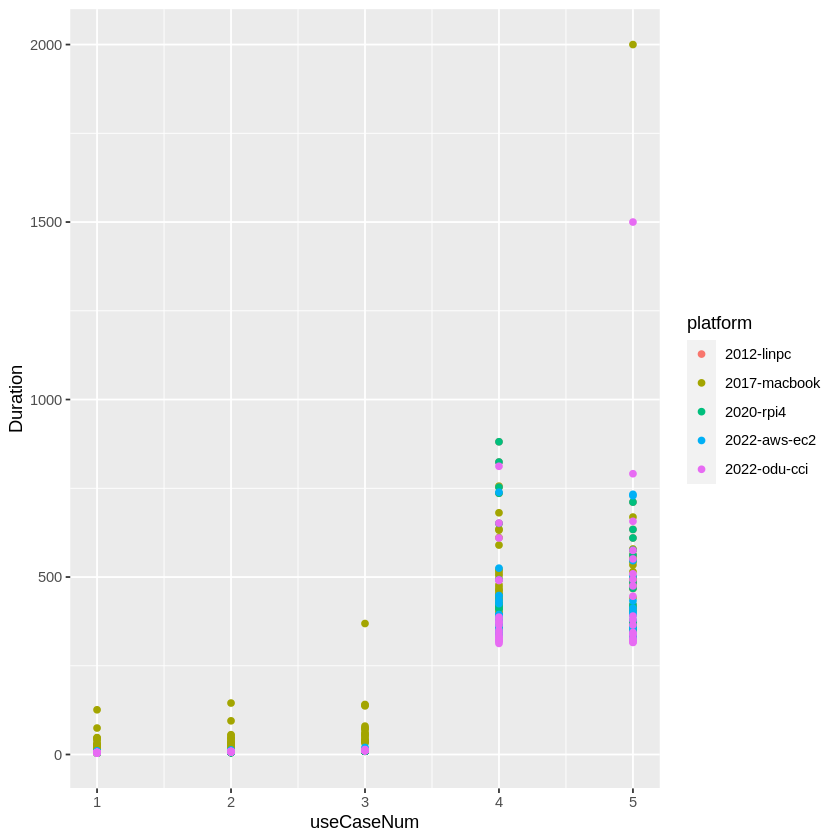
\includegraphics{dss-span-analysis-rev5_files/figure-pdf/cell-22-output-1.png}

}

\end{figure}

\hypertarget{remove-macbook-data-from-development-platform}{%
\subsection{Remove Macbook Data from Development
Platform}\label{remove-macbook-data-from-development-platform}}

Here we remove the data from the Macbook development platform. The qplot
shows that the \textbf{Mac implementation of Docker} adds latency within
the Docker environment. In non-linux based plaforms, a Docker desktop
running a virtual machine is required to provided that Docker capability
that is native to Linux platforms. The Mac is considered to be the
development environment and not representative of the integration and
production environments.

https://dev.to/ericnograles/why-is-docker-on-macos-so-much-worse-than-linux-flh\\
https://collabnix.com/how-docker-for-mac-works-under-the-hood/

\begin{Shaded}
\begin{Highlighting}[]
\NormalTok{noMacSpan }\OtherTok{\textless{}{-}}\NormalTok{ spanMetricsA[}\SpecialCharTok{!}\NormalTok{spanMetricsA}\SpecialCharTok{$}\NormalTok{env }\SpecialCharTok{==} \DecValTok{0}\NormalTok{,]}
\end{Highlighting}
\end{Shaded}

\begin{Shaded}
\begin{Highlighting}[]
\FunctionTok{qplot}\NormalTok{(useCaseNum, Duration, }\AttributeTok{data =}\NormalTok{ noMacSpan, }\AttributeTok{colour =}\NormalTok{ platform)}
\end{Highlighting}
\end{Shaded}

\begin{figure}[H]

{\centering 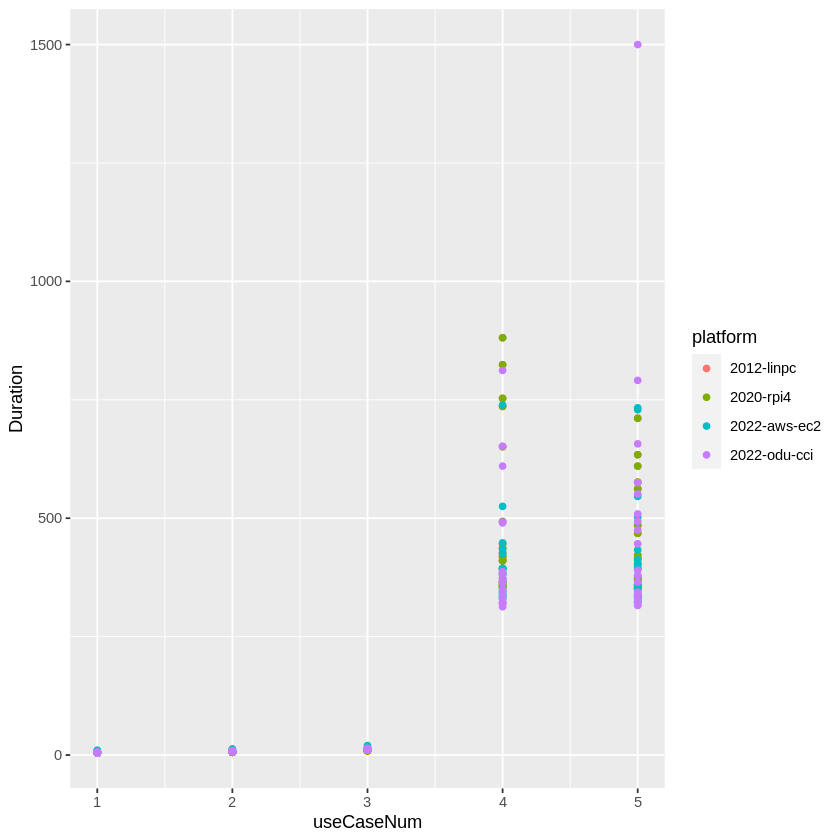
\includegraphics{dss-span-analysis-rev5_files/figure-pdf/cell-24-output-1.png}

}

\end{figure}

\begin{Shaded}
\begin{Highlighting}[]
\CommentTok{\# par(mfrow=c(2,1))}
\CommentTok{\# hist(spanMetricsA$Duration, counts = 5)}

\CommentTok{\# spanMetricsA \%\textgreater{}\%}
\CommentTok{\#     ggplot(aes(Trace.name, Duration)) + }
\CommentTok{\#     stat\_boxplot(notch="FALSE") + geom\_point() +}
\CommentTok{\#     ggtitle("Duration of Endpoint Responses from Trace")}
\CommentTok{\# \# notch went outside hinges. Try setting notch=FALSE.}
\end{Highlighting}
\end{Shaded}

\begin{Shaded}
\begin{Highlighting}[]
\CommentTok{\# Remove outliers}
\NormalTok{aSpan }\OtherTok{\textless{}{-}}\NormalTok{ noMacSpan}
\NormalTok{outliers }\OtherTok{\textless{}{-}} \FunctionTok{boxplot}\NormalTok{(aSpan}\SpecialCharTok{$}\NormalTok{Duration, }\AttributeTok{plot =} \ConstantTok{FALSE}\NormalTok{)}\SpecialCharTok{$}\NormalTok{out}
\NormalTok{outliers}

\NormalTok{aSpan }\OtherTok{\textless{}{-}}\NormalTok{ aSpan[}\SpecialCharTok{{-}}\FunctionTok{which}\NormalTok{(aSpan}\SpecialCharTok{$}\NormalTok{Duration }\SpecialCharTok{\%in\%}\NormalTok{ outliers),]}
\end{Highlighting}
\end{Shaded}

1500

\begin{Shaded}
\begin{Highlighting}[]
\NormalTok{aSpan }\SpecialCharTok{\%\textgreater{}\%}
    \FunctionTok{ggplot}\NormalTok{(}\FunctionTok{aes}\NormalTok{(Trace.name, Duration)) }\SpecialCharTok{+} 
    \FunctionTok{stat\_boxplot}\NormalTok{(}\AttributeTok{notch=}\StringTok{"FALSE"}\NormalTok{) }\SpecialCharTok{+} \FunctionTok{geom\_point}\NormalTok{(}\FunctionTok{aes}\NormalTok{(}\AttributeTok{colour =}\NormalTok{ platform)) }\SpecialCharTok{+}
    \FunctionTok{ggtitle}\NormalTok{(}\StringTok{"Trace Duration (ms) (Outliers Removed)"}\NormalTok{) }\SpecialCharTok{+}
    \FunctionTok{ylab}\NormalTok{(}\StringTok{"Duration (ms)"}\NormalTok{) }\SpecialCharTok{+}
    \FunctionTok{xlab}\NormalTok{(}\StringTok{"DSS Use Case (i.e., Trace.name)"}\NormalTok{)}
\CommentTok{\# notch went outside hinges. Try setting notch=FALSE.}
\end{Highlighting}
\end{Shaded}

\begin{figure}[H]

{\centering 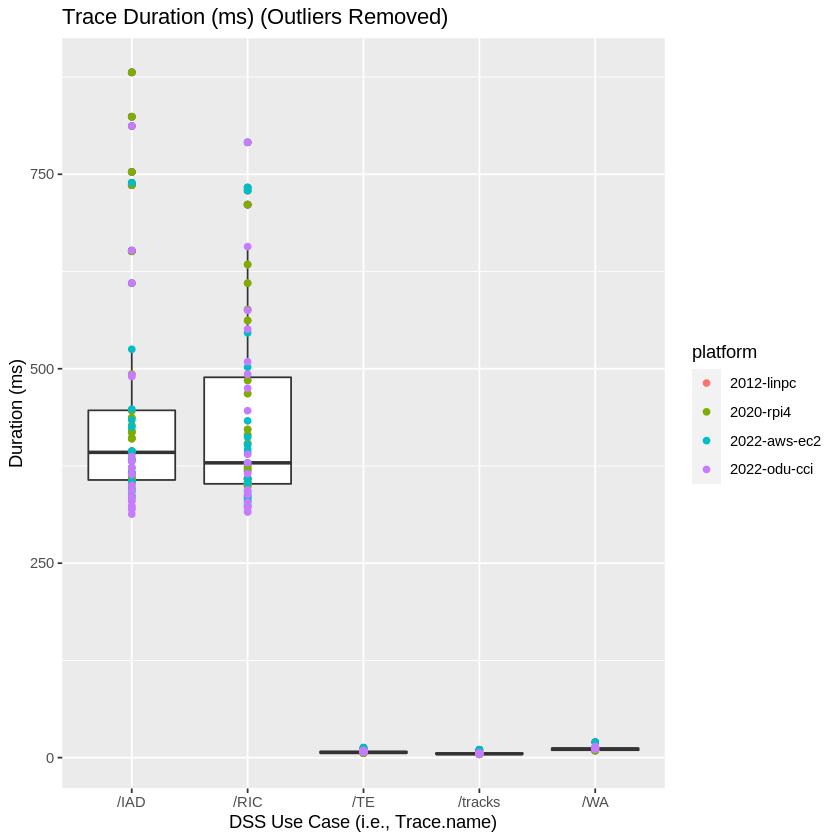
\includegraphics{dss-span-analysis-rev5_files/figure-pdf/cell-27-output-1.png}

}

\end{figure}

\begin{Shaded}
\begin{Highlighting}[]
\NormalTok{aSpan }\SpecialCharTok{\%\textgreater{}\%}
    \FunctionTok{ggplot}\NormalTok{(}\FunctionTok{aes}\NormalTok{(Duration)) }\SpecialCharTok{+} \FunctionTok{geom\_histogram}\NormalTok{(}\AttributeTok{binwidth =} \DecValTok{20}\NormalTok{) }\SpecialCharTok{+}
    \FunctionTok{ggtitle}\NormalTok{(}\StringTok{"Duration (ms) Histogram (Outliers Removed), Binwidth = 20"}\NormalTok{) }\SpecialCharTok{+}
    \FunctionTok{xlab}\NormalTok{(}\StringTok{"Duration (ms)"}\NormalTok{)}
\end{Highlighting}
\end{Shaded}

\begin{figure}[H]

{\centering 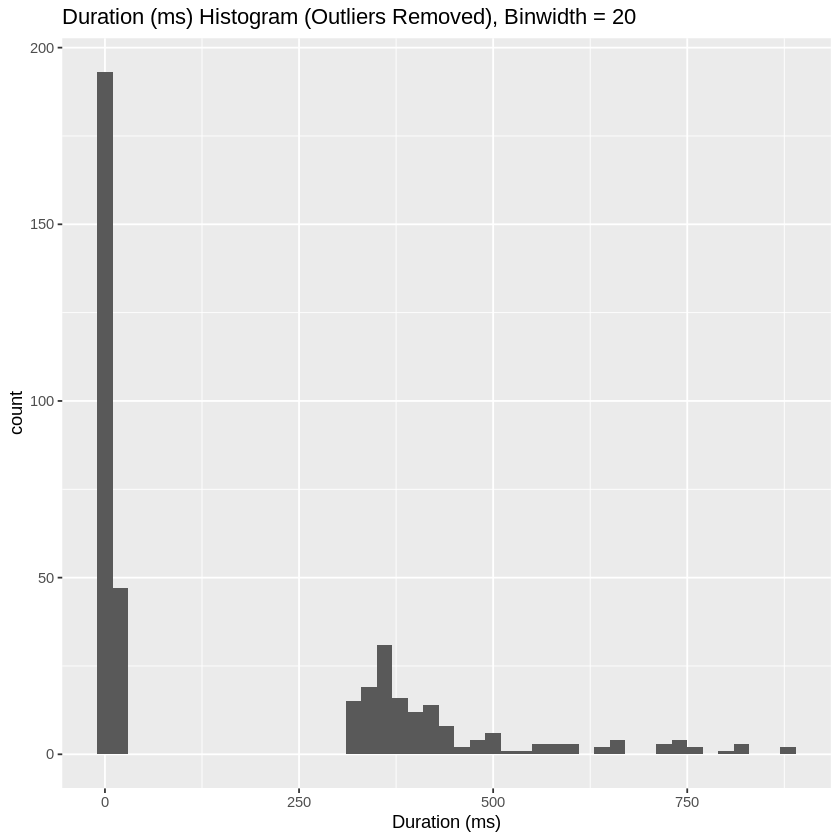
\includegraphics{dss-span-analysis-rev5_files/figure-pdf/cell-28-output-1.png}

}

\end{figure}

\begin{Shaded}
\begin{Highlighting}[]
\FunctionTok{summary}\NormalTok{(aSpan)}
\FunctionTok{sd}\NormalTok{(aSpan}\SpecialCharTok{$}\NormalTok{Duration)}
\end{Highlighting}
\end{Shaded}

\begin{verbatim}
   Trace.ID          Trace.name         Start.time           Duration      
 Length:399         Length:399         Length:399         Min.   :  4.290  
 Class :character   Class :character   Class :character   1st Qu.:  6.045  
 Mode  :character   Mode  :character   Mode  :character   Median : 11.100  
                                                          Mean   :180.874  
                                                          3rd Qu.:364.500  
                                                          Max.   :881.000  
   platform              env          useCase            useCaseNum   
 Length:399         Min.   :1.000   Length:399         Min.   :1.000  
 Class :character   1st Qu.:1.500   Class :character   1st Qu.:2.000  
 Mode  :character   Median :2.000   Mode  :character   Median :3.000  
                    Mean   :2.496                      Mean   :2.995  
                    3rd Qu.:3.000                      3rd Qu.:4.000  
                    Max.   :4.000                      Max.   :5.000  
    ext             V10         
 Mode :logical   Mode :logical  
 FALSE:240       FALSE:34       
 TRUE :159       TRUE :365      
                                
                                
                                
\end{verbatim}

229.448905568277

\begin{Shaded}
\begin{Highlighting}[]
\CommentTok{\# dnorm\_aSpan \textless{}{-} aSpan}
\CommentTok{\# dnorm\_aSpan$Duration \textless{}{-} dnorm(dnorm\_aSpan$Duration,mean=180.874,sd=229.4489)}

\CommentTok{\# dnorm\_aSpan \%\textgreater{}\%}
\CommentTok{\#     ggplot(aes(Duration)) + geom\_histogram() +}
\CommentTok{\#     ggtitle("Duration (ms) Histogram (w dnorm, Binwidth = 20") +}
\CommentTok{\#     xlab("Duration (ms)")}

\CommentTok{\# shapiro.test(dnorm\_aSpan$Duration)}
\end{Highlighting}
\end{Shaded}

\begin{Shaded}
\begin{Highlighting}[]
\CommentTok{\# ggpairs(spanMetricsNum, title="correlogram with ggpairs()")}
\end{Highlighting}
\end{Shaded}

\hypertarget{mclust}{%
\subsubsection{mclust}\label{mclust}}

Used mclust to verify the separation of internal and external models as
indicated from the useCaseNum vs.~Duration plot; i.e.~use cases 4 and 5
use an external API.

The library mclust is a contributed R package for model-based
clustering, classification, and density estimation based on finite
normal mixture modelling. It provides functions for parameter estimation
via the EM algorithm for normal mixture models with a variety of
covariance structures, and functions for simulation from these models.

\emph{Scrucca L., Fop M., Murphy T. B. and Raftery A. E. (2016) mclust
5: clustering, classification and density estimation using Gaussian
finite mixture models The R Journal 8/1, pp.~289-317}

\begin{Shaded}
\begin{Highlighting}[]
\FunctionTok{install.packages}\NormalTok{(}\StringTok{"mclust"}\NormalTok{)}
\FunctionTok{library}\NormalTok{(mclust, }\AttributeTok{quietly =} \ConstantTok{TRUE}\NormalTok{)}
\end{Highlighting}
\end{Shaded}

\hypertarget{mclust-univariate-analysis-of-duration}{%
\subsubsection{Mclust Univariate Analysis of
Duration}\label{mclust-univariate-analysis-of-duration}}

\begin{Shaded}
\begin{Highlighting}[]
\NormalTok{mod4 }\OtherTok{\textless{}{-}} \FunctionTok{densityMclust}\NormalTok{(aSpan}\SpecialCharTok{$}\NormalTok{Duration)}
\end{Highlighting}
\end{Shaded}

\begin{figure}[H]

{\centering 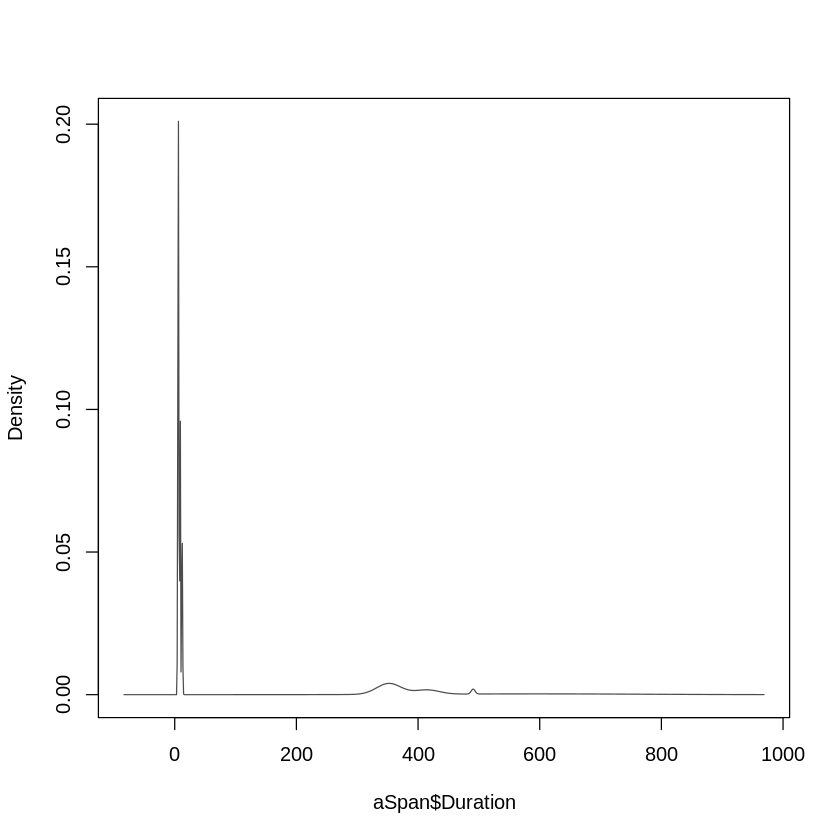
\includegraphics{dss-span-analysis-rev5_files/figure-pdf/cell-33-output-1.png}

}

\end{figure}

\begin{Shaded}
\begin{Highlighting}[]
\FunctionTok{summary}\NormalTok{(mod4)}
\end{Highlighting}
\end{Shaded}

\begin{verbatim}
------------------------------------------------------- 
Density estimation via Gaussian finite mixture modeling 
------------------------------------------------------- 

Mclust V (univariate, unequal variance) model with 9 components: 

 log-likelihood   n df       BIC       ICL
      -1656.953 399 26 -3469.619 -3511.198
\end{verbatim}

\begin{Shaded}
\begin{Highlighting}[]
\FunctionTok{plot}\NormalTok{(mod4, }\AttributeTok{what =}\StringTok{"BIC"}\NormalTok{)}
\end{Highlighting}
\end{Shaded}

\begin{figure}[H]

{\centering 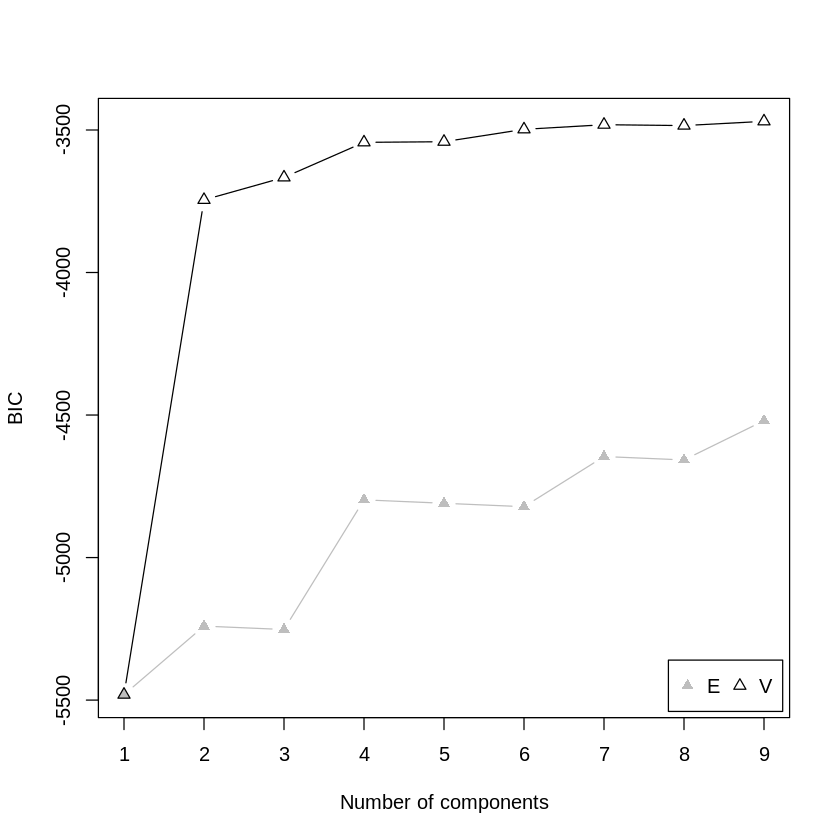
\includegraphics{dss-span-analysis-rev5_files/figure-pdf/cell-35-output-1.png}

}

\end{figure}

\begin{Shaded}
\begin{Highlighting}[]
\FunctionTok{plot}\NormalTok{(mod4, }\AttributeTok{what =} \StringTok{"density"}\NormalTok{, }\AttributeTok{data =}\NormalTok{ aSpan}\SpecialCharTok{$}\NormalTok{Duration, }\AttributeTok{breaks =} \DecValTok{20}\NormalTok{)}
\end{Highlighting}
\end{Shaded}

\begin{figure}[H]

{\centering 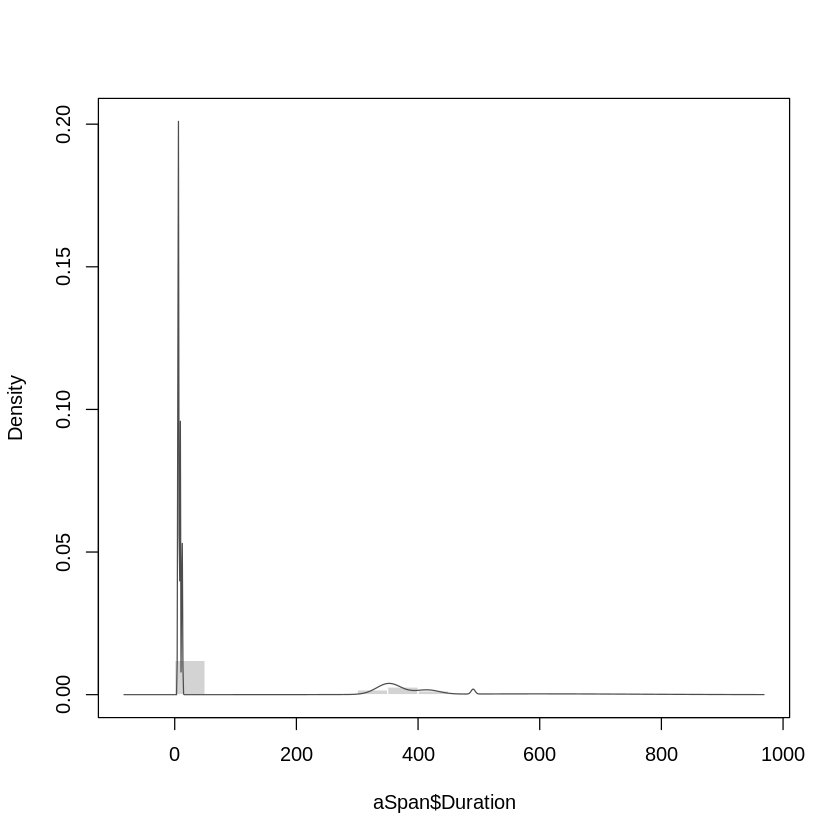
\includegraphics{dss-span-analysis-rev5_files/figure-pdf/cell-36-output-1.png}

}

\end{figure}

\begin{Shaded}
\begin{Highlighting}[]
\FunctionTok{plot}\NormalTok{(mod4, }\AttributeTok{what =} \StringTok{"diagnostic"}\NormalTok{, }\AttributeTok{type =} \StringTok{"cdf"}\NormalTok{)}
\end{Highlighting}
\end{Shaded}

\begin{figure}[H]

{\centering 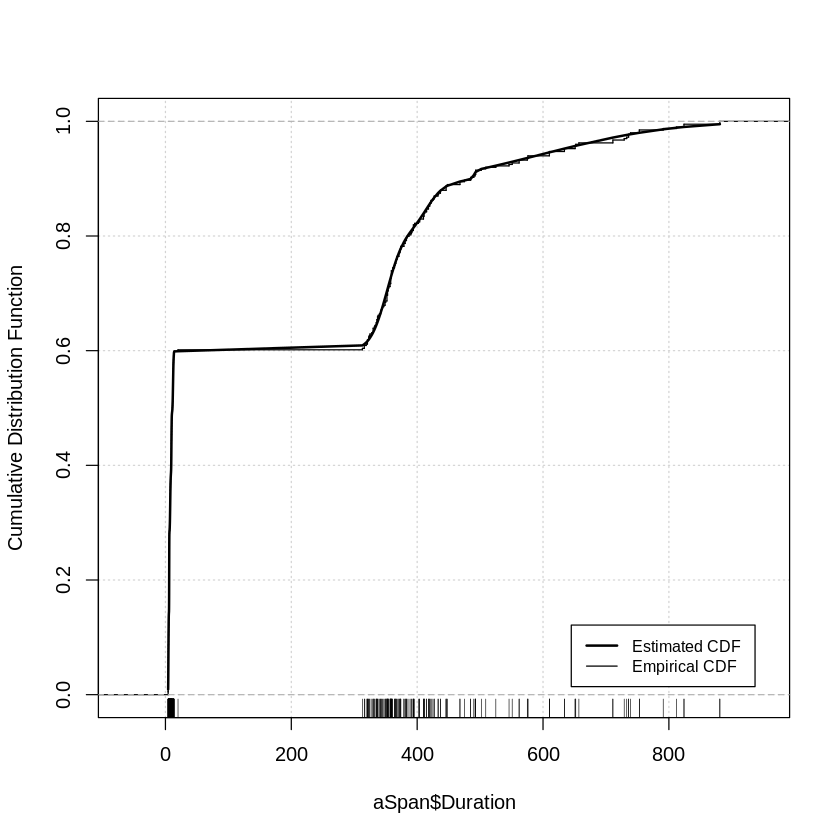
\includegraphics{dss-span-analysis-rev5_files/figure-pdf/cell-37-output-1.png}

}

\end{figure}

\begin{Shaded}
\begin{Highlighting}[]
\FunctionTok{plot}\NormalTok{(mod4, }\AttributeTok{what =} \StringTok{"diagnostic"}\NormalTok{, }\AttributeTok{type =} \StringTok{"qq"}\NormalTok{)}
\end{Highlighting}
\end{Shaded}

\begin{figure}[H]

{\centering 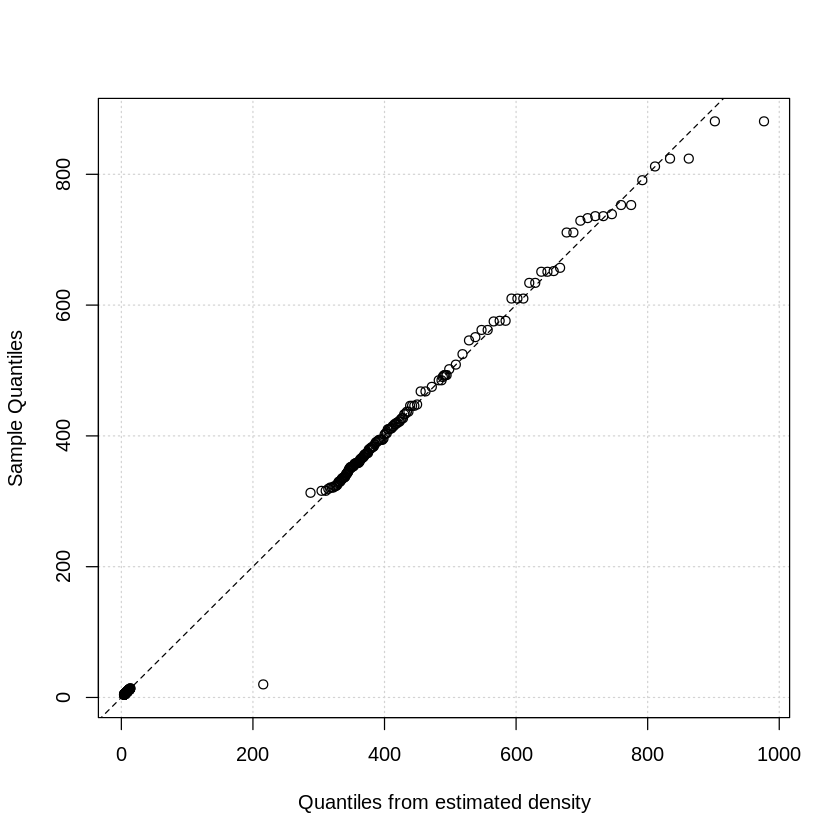
\includegraphics{dss-span-analysis-rev5_files/figure-pdf/cell-38-output-1.png}

}

\end{figure}

\hypertarget{mclust-multivariate-analysis}{%
\subsubsection{Mclust Multivariate
Analysis}\label{mclust-multivariate-analysis}}

\begin{Shaded}
\begin{Highlighting}[]
\NormalTok{uc }\OtherTok{\textless{}{-}}\NormalTok{ aSpan}\SpecialCharTok{$}\NormalTok{useCaseNum }\CommentTok{\# Trace.name is char, used uc num conversion}

\NormalTok{X }\OtherTok{\textless{}{-}}\NormalTok{ aSpan }\SpecialCharTok{\%\textgreater{}\%}
    \CommentTok{\# dplyr::select(useCaseNum, env, ext, Duration)}
\NormalTok{    dplyr}\SpecialCharTok{::}\FunctionTok{select}\NormalTok{(Duration, ext, env)}
    \CommentTok{\# dplyr::select(Duration)}

\FunctionTok{head}\NormalTok{(X)}
\FunctionTok{clPairs}\NormalTok{(X, uc)}
\end{Highlighting}
\end{Shaded}

A data.frame: 6 × 3

\begin{longtable}[]{@{}llll@{}}
\toprule()
& Duration \textless dbl\textgreater{} & ext \textless lgl\textgreater{}
& env \textless dbl\textgreater{} \\
\midrule()
\endhead
21 & 4.90 & FALSE & 1 \\
22 & 4.43 & FALSE & 1 \\
23 & 4.67 & FALSE & 1 \\
24 & 4.68 & FALSE & 1 \\
25 & 4.73 & FALSE & 1 \\
26 & 4.89 & FALSE & 1 \\
\bottomrule()
\end{longtable}

\begin{figure}[H]

{\centering 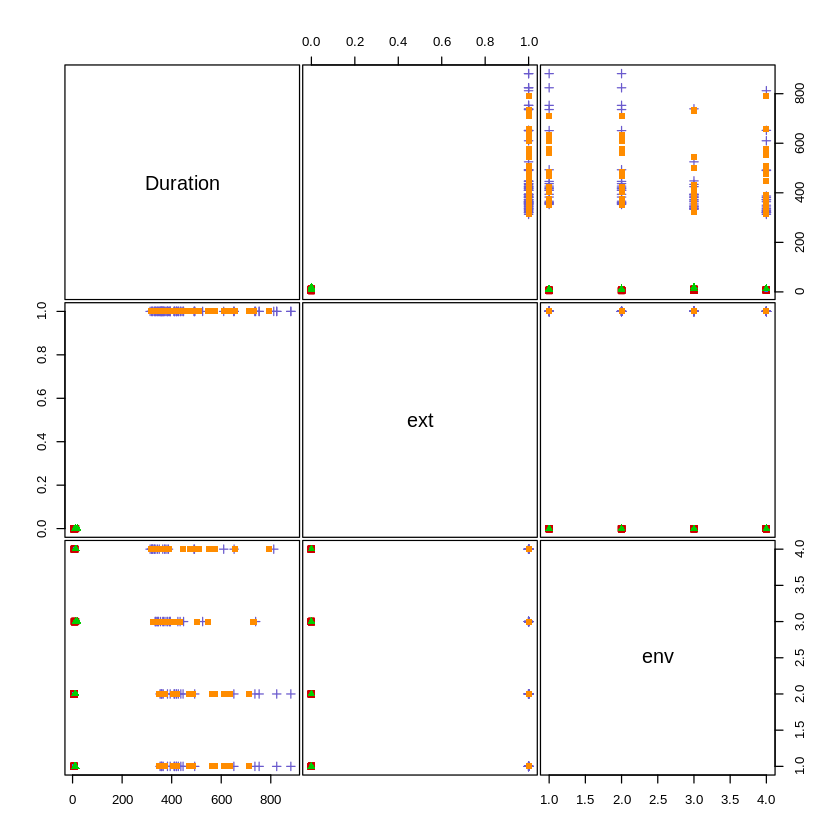
\includegraphics{dss-span-analysis-rev5_files/figure-pdf/cell-39-output-2.png}

}

\end{figure}

\begin{Shaded}
\begin{Highlighting}[]
\CommentTok{\# spanMclust \textless{}{-} Mclust(aSpan)}
\CommentTok{\# spanMclust \textless{}{-} Mclust(X)}
\CommentTok{\# summary(spanMclust)}
\CommentTok{\# plot(spanMclust, what = c("classification"))}
\end{Highlighting}
\end{Shaded}

\begin{Shaded}
\begin{Highlighting}[]
\NormalTok{BIC }\OtherTok{\textless{}{-}} \FunctionTok{mclustBIC}\NormalTok{(X)}
\FunctionTok{plot}\NormalTok{(BIC)}
\end{Highlighting}
\end{Shaded}

\begin{figure}[H]

{\centering 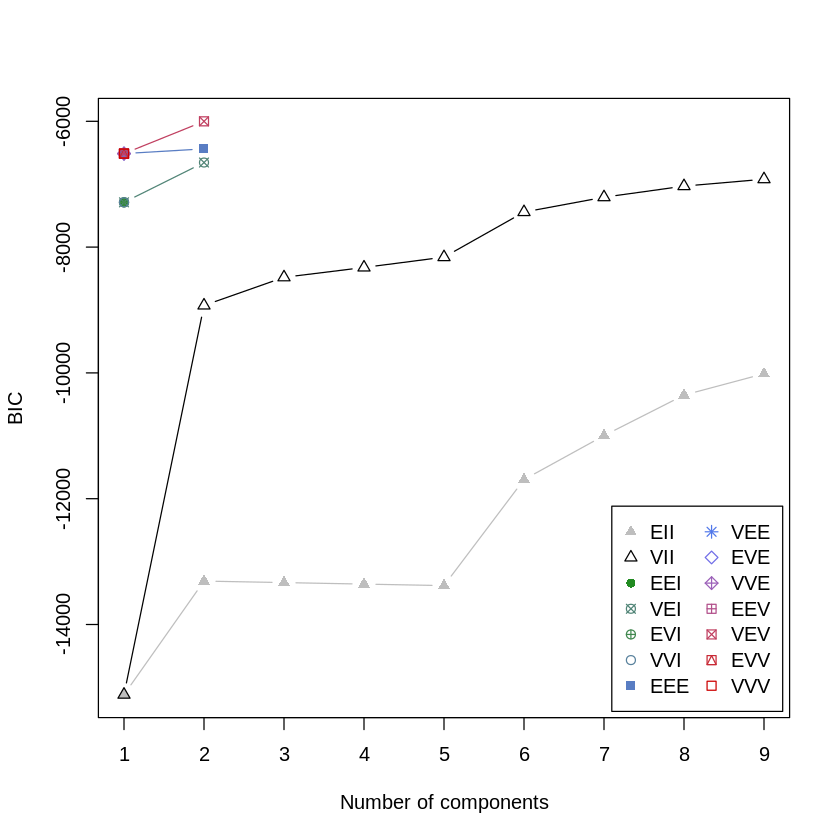
\includegraphics{dss-span-analysis-rev5_files/figure-pdf/cell-41-output-1.png}

}

\end{figure}

\begin{Shaded}
\begin{Highlighting}[]
\FunctionTok{summary}\NormalTok{(BIC)}
\end{Highlighting}
\end{Shaded}

\begin{verbatim}
Best BIC values:
             VEV,2      EEE,2      EEE,1
BIC      -6000.192 -6437.9228 -6512.9492
BIC diff     0.000  -437.7311  -512.7575
\end{verbatim}

Note that 2 is included within the list of best Bayesian Information
Criterion (BIC) values.

\begin{Shaded}
\begin{Highlighting}[]
\CommentTok{\# mod1 \textless{}{-} Mclust(X, x = BIC)}
\CommentTok{\# summary(mod1, parameters = TRUE)}
\end{Highlighting}
\end{Shaded}

\begin{Shaded}
\begin{Highlighting}[]
\CommentTok{\# plot(mod1, what = "classification")}
\end{Highlighting}
\end{Shaded}

\begin{Shaded}
\begin{Highlighting}[]
\CommentTok{\# plot(mod1, what = "uncertainty")}
\end{Highlighting}
\end{Shaded}

\begin{Shaded}
\begin{Highlighting}[]
\CommentTok{\# ICL \textless{}{-} mclustICL(X)}
\CommentTok{\# summary(ICL)}
\CommentTok{\# plot(ICL)}
\end{Highlighting}
\end{Shaded}

\begin{Shaded}
\begin{Highlighting}[]
\CommentTok{\# LRT \textless{}{-} mclustBootstrapLRT(X, modelName = "VEV")}
\CommentTok{\# LRT}
\end{Highlighting}
\end{Shaded}

\begin{Shaded}
\begin{Highlighting}[]
\FunctionTok{qqnorm}\NormalTok{(aSpan}\SpecialCharTok{$}\NormalTok{Duration, }\AttributeTok{main=}\StringTok{"Span Duration Q{-}Q Norm Plot"}\NormalTok{)}
\FunctionTok{qqline}\NormalTok{(aSpan}\SpecialCharTok{$}\NormalTok{Duration)}
\end{Highlighting}
\end{Shaded}

\begin{figure}[H]

{\centering 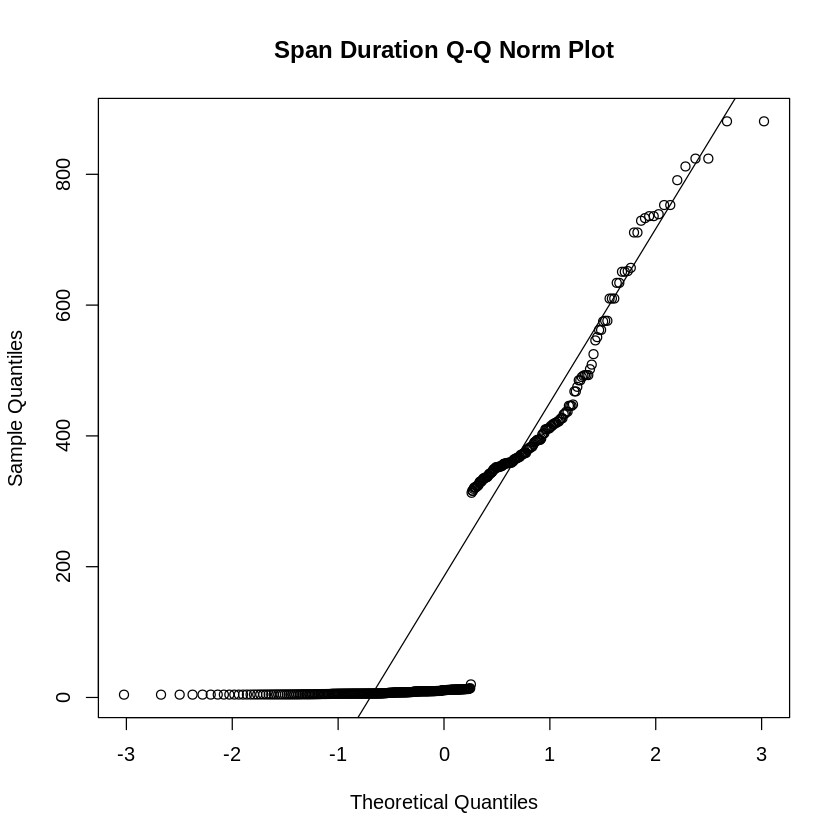
\includegraphics{dss-span-analysis-rev5_files/figure-pdf/cell-48-output-1.png}

}

\end{figure}

\begin{Shaded}
\begin{Highlighting}[]
\CommentTok{\# head(aSpan)}
\end{Highlighting}
\end{Shaded}

\begin{Shaded}
\begin{Highlighting}[]
\NormalTok{aSpan\_Density }\OtherTok{\textless{}{-}}\NormalTok{ aSpan }\SpecialCharTok{\%\textgreater{}\%}
    \CommentTok{\# dplyr::select(useCaseNum, env, ext, Duration)}
\NormalTok{    dplyr}\SpecialCharTok{::}\FunctionTok{select}\NormalTok{(ext, Duration)}
    \CommentTok{\# dplyr::select(Duration)}
\end{Highlighting}
\end{Shaded}

\begin{Shaded}
\begin{Highlighting}[]
\NormalTok{mod5 }\OtherTok{\textless{}{-}} \FunctionTok{densityMclust}\NormalTok{(aSpan\_Density)}
\end{Highlighting}
\end{Shaded}

\begin{figure}[H]

{\centering 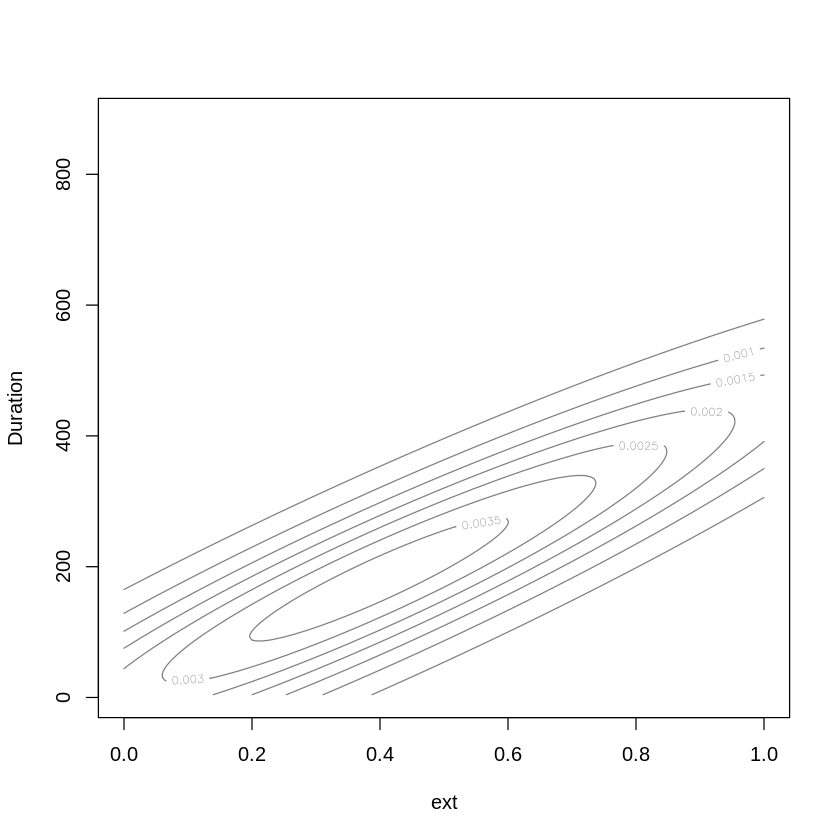
\includegraphics{dss-span-analysis-rev5_files/figure-pdf/cell-51-output-1.png}

}

\end{figure}

\hypertarget{separating-internal-from-external-data}{%
\section{Separating Internal from External
Data}\label{separating-internal-from-external-data}}

\hypertarget{internal-data}{%
\subsection{Internal Data}\label{internal-data}}

\begin{Shaded}
\begin{Highlighting}[]
\CommentTok{\# Separate Internal Data}
\CommentTok{\# Could use ext == FALSE}

\NormalTok{tracksSpanData }\OtherTok{=} \FunctionTok{subset}\NormalTok{(aSpan, useCaseNum }\SpecialCharTok{==} \DecValTok{1}\NormalTok{)}
\NormalTok{TE\_SpanData }\OtherTok{=} \FunctionTok{subset}\NormalTok{(aSpan, useCaseNum }\SpecialCharTok{==} \DecValTok{2}\NormalTok{)}
\NormalTok{WA\_SpanData }\OtherTok{=} \FunctionTok{subset}\NormalTok{(aSpan, useCaseNum }\SpecialCharTok{==} \DecValTok{3}\NormalTok{)}

\NormalTok{internalSpanData }\OtherTok{\textless{}{-}} \FunctionTok{rbind}\NormalTok{(tracksSpanData, TE\_SpanData, WA\_SpanData)}
\NormalTok{dssSpanData }\OtherTok{\textless{}{-}} \FunctionTok{rbind}\NormalTok{(TE\_SpanData, WA\_SpanData)}
\end{Highlighting}
\end{Shaded}

\begin{Shaded}
\begin{Highlighting}[]
\CommentTok{\# Remove Outliers}
\CommentTok{\# outliers \textless{}{-} boxplot(internalSpanData$Duration, plot = FALSE)$out}
\CommentTok{\# outliers}
\CommentTok{\# iSpan \textless{}{-} iSpan[{-}which(iSpan$Duration \%in\% outliers),]}

\NormalTok{outliers }\OtherTok{\textless{}{-}} \FunctionTok{which}\NormalTok{(internalSpanData}\SpecialCharTok{$}\NormalTok{Duration }\SpecialCharTok{\textgreater{}} \DecValTok{50}\NormalTok{) }\CommentTok{\#outlier rows}
\NormalTok{outliers}
\CommentTok{\# iSpan \textless{}{-} internalSpanData[!outliers,]}
\CommentTok{\# iSpan \textless{}{-} dssSpanData[!dssSpanData$Duration \textgreater{} 50,]}
\NormalTok{iSpan }\OtherTok{\textless{}{-}}\NormalTok{ internalSpanData[}\SpecialCharTok{!}\NormalTok{internalSpanData}\SpecialCharTok{$}\NormalTok{Duration }\SpecialCharTok{\textgreater{}} \DecValTok{50}\NormalTok{,]}
    \CommentTok{\# Remove if duration is greater than a value}

\CommentTok{\# iSpan}
\end{Highlighting}
\end{Shaded}

\begin{Shaded}
\begin{Highlighting}[]
\FunctionTok{summary}\NormalTok{(iSpan)}
\FunctionTok{sd}\NormalTok{(iSpan}\SpecialCharTok{$}\NormalTok{Duration)}
\end{Highlighting}
\end{Shaded}

\begin{verbatim}
   Trace.ID          Trace.name         Start.time           Duration     
 Length:240         Length:240         Length:240         Min.   : 4.290  
 Class :character   Class :character   Class :character   1st Qu.: 5.713  
 Mode  :character   Mode  :character   Mode  :character   Median : 7.070  
                                                          Mean   : 7.745  
                                                          3rd Qu.: 9.610  
                                                          Max.   :20.000  
   platform              env         useCase            useCaseNum
 Length:240         Min.   :1.00   Length:240         Min.   :1   
 Class :character   1st Qu.:1.75   Class :character   1st Qu.:1   
 Mode  :character   Median :2.50   Mode  :character   Median :2   
                    Mean   :2.50                      Mean   :2   
                    3rd Qu.:3.25                      3rd Qu.:3   
                    Max.   :4.00                      Max.   :3   
    ext            V10         
 Mode :logical   Mode:logical  
 FALSE:240       TRUE:240      
                               
                               
                               
                               
\end{verbatim}

2.77664210997812

\begin{Shaded}
\begin{Highlighting}[]
\NormalTok{iSpan }\SpecialCharTok{\%\textgreater{}\%}
    \FunctionTok{ggplot}\NormalTok{(}\FunctionTok{aes}\NormalTok{(Trace.name, Duration)) }\SpecialCharTok{+} 
    \FunctionTok{stat\_boxplot}\NormalTok{(}\AttributeTok{notch=}\StringTok{"TRUE"}\NormalTok{) }\SpecialCharTok{+} \FunctionTok{geom\_point}\NormalTok{(}\FunctionTok{aes}\NormalTok{(}\AttributeTok{colour =}\NormalTok{ platform)) }\SpecialCharTok{+}
    \FunctionTok{ggtitle}\NormalTok{(}\StringTok{"Internal Trace Duration (ms) (Outliers Removed)"}\NormalTok{) }\SpecialCharTok{+}
    \FunctionTok{ylab}\NormalTok{(}\StringTok{"Duration (ms)"}\NormalTok{) }\SpecialCharTok{+}
    \FunctionTok{xlab}\NormalTok{(}\StringTok{"DSS Use Case (i.e., Trace.name)"}\NormalTok{)}
\end{Highlighting}
\end{Shaded}

\begin{figure}[H]

{\centering 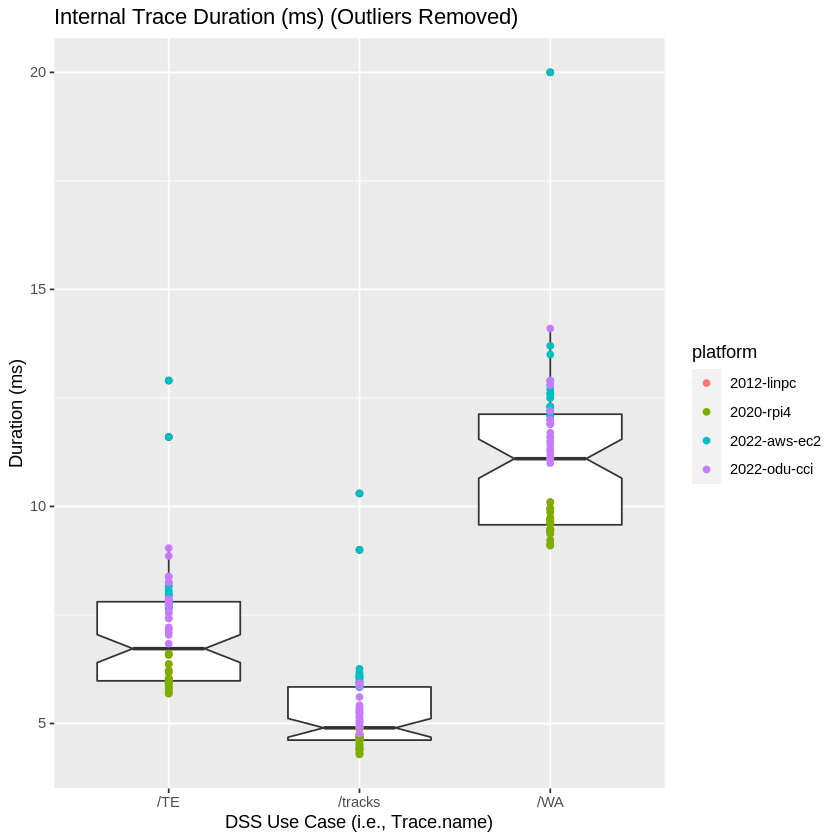
\includegraphics{dss-span-analysis-rev5_files/figure-pdf/cell-55-output-1.png}

}

\end{figure}

\begin{Shaded}
\begin{Highlighting}[]
\NormalTok{iSpan }\SpecialCharTok{\%\textgreater{}\%}
    \FunctionTok{ggplot}\NormalTok{(}\FunctionTok{aes}\NormalTok{(Duration)) }\SpecialCharTok{+} \FunctionTok{geom\_histogram}\NormalTok{(}\AttributeTok{binwidth =} \DecValTok{1}\NormalTok{) }\SpecialCharTok{+}
    \FunctionTok{ggtitle}\NormalTok{(}\StringTok{"Internal Duration (ms) Histogram (Outliers Removed), Binwidth = 1ms"}\NormalTok{) }\SpecialCharTok{+}
    \FunctionTok{xlab}\NormalTok{(}\StringTok{"Internal Duration (ms)"}\NormalTok{)}
\end{Highlighting}
\end{Shaded}

\begin{figure}[H]

{\centering 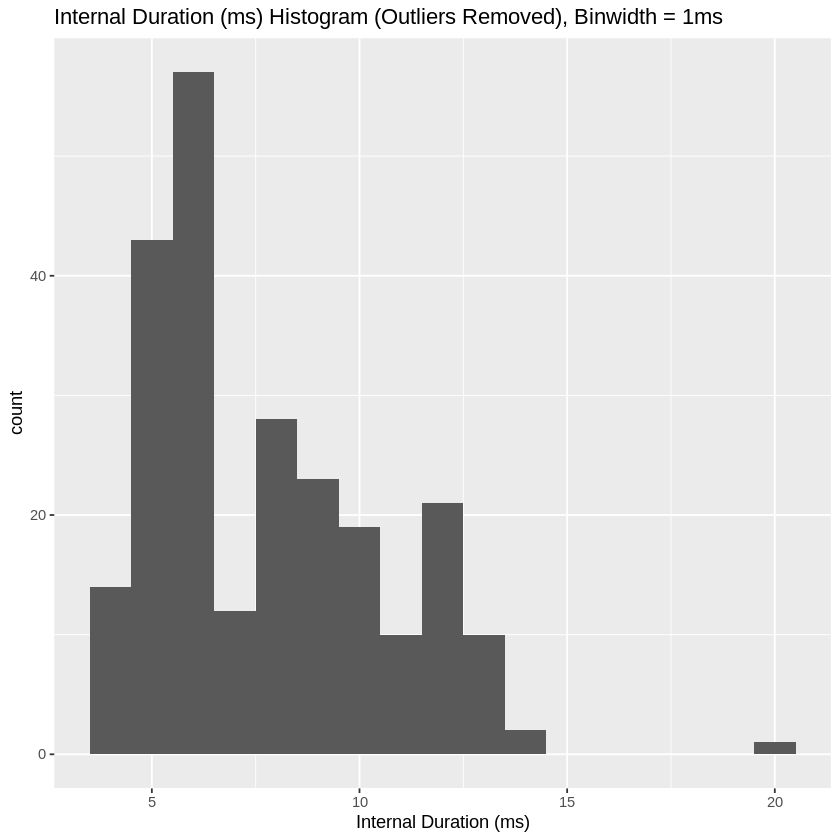
\includegraphics{dss-span-analysis-rev5_files/figure-pdf/cell-56-output-1.png}

}

\end{figure}

\begin{Shaded}
\begin{Highlighting}[]
\CommentTok{\# dnorm\_iSpan \textless{}{-} iSpan}
\CommentTok{\# dnorm\_iSpan$Duration \textless{}{-} dnorm(dnorm\_iSpan$Duration,mean=7.745,sd=2.776)}

\CommentTok{\# dnorm\_iSpan \%\textgreater{}\%}
\CommentTok{\#     ggplot(aes(Duration)) + geom\_histogram() +}
\CommentTok{\#     ggtitle("Duration (ms) Histogram (w dnorm, Binwidth = auto") +}
\CommentTok{\#     xlab("Duration (ms)")}

\CommentTok{\# shapiro.test(dnorm\_iSpan$Duration)}
\end{Highlighting}
\end{Shaded}

Note that the histogram plot indicates that the data is not normally
distrbuted and will need a transformation to enable application of
statistics.

\hypertarget{external-data}{%
\subsection{External Data}\label{external-data}}

\begin{Shaded}
\begin{Highlighting}[]
\NormalTok{RIC\_SpanData }\OtherTok{=} \FunctionTok{subset}\NormalTok{(aSpan, useCaseNum }\SpecialCharTok{==} \DecValTok{5}\NormalTok{)}
\NormalTok{IAD\_SpanData }\OtherTok{=} \FunctionTok{subset}\NormalTok{(aSpan, useCaseNum }\SpecialCharTok{==} \DecValTok{4}\NormalTok{)}

\NormalTok{externalSpanData }\OtherTok{\textless{}{-}} \FunctionTok{rbind}\NormalTok{(RIC\_SpanData, IAD\_SpanData)}
\end{Highlighting}
\end{Shaded}

\begin{Shaded}
\begin{Highlighting}[]
\CommentTok{\# Remove outliers}
\CommentTok{\# outliers \textless{}{-} boxplot(externalSpanData$Duration, plot = FALSE)$out}
\CommentTok{\# outliers}

\NormalTok{eSpan }\OtherTok{\textless{}{-}}\NormalTok{ externalSpanData}
\CommentTok{\# eSpan \textless{}{-} eSpan[{-}which(eSpan$Duration \%in\% outliers),]}
\end{Highlighting}
\end{Shaded}

\begin{Shaded}
\begin{Highlighting}[]
\FunctionTok{summary}\NormalTok{(eSpan)}
\FunctionTok{sd}\NormalTok{(eSpan}\SpecialCharTok{$}\NormalTok{Duration)}
\end{Highlighting}
\end{Shaded}

\begin{verbatim}
   Trace.ID          Trace.name         Start.time           Duration    
 Length:159         Length:159         Length:159         Min.   :313.0  
 Class :character   Class :character   Class :character   1st Qu.:353.0  
 Mode  :character   Mode  :character   Mode  :character   Median :387.0  
                                                          Mean   :442.2  
                                                          3rd Qu.:485.0  
                                                          Max.   :881.0  
   platform              env          useCase            useCaseNum   
 Length:159         Min.   :1.000   Length:159         Min.   :4.000  
 Class :character   1st Qu.:1.500   Class :character   1st Qu.:4.000  
 Mode  :character   Median :2.000   Mode  :character   Median :4.000  
                    Mean   :2.491                      Mean   :4.497  
                    3rd Qu.:3.000                      3rd Qu.:5.000  
                    Max.   :4.000                      Max.   :5.000  
   ext             V10         
 Mode:logical   Mode :logical  
 TRUE:159       FALSE:34       
                TRUE :125      
                               
                               
                               
\end{verbatim}

135.466366505137

\begin{Shaded}
\begin{Highlighting}[]
\NormalTok{eSpan }\SpecialCharTok{\%\textgreater{}\%}
    \FunctionTok{ggplot}\NormalTok{(}\FunctionTok{aes}\NormalTok{(Trace.name, Duration)) }\SpecialCharTok{+} 
    \FunctionTok{stat\_boxplot}\NormalTok{(}\AttributeTok{notch=}\StringTok{"TRUE"}\NormalTok{) }\SpecialCharTok{+} \FunctionTok{geom\_point}\NormalTok{(}\FunctionTok{aes}\NormalTok{(}\AttributeTok{colour =}\NormalTok{ platform)) }\SpecialCharTok{+}
    \FunctionTok{ggtitle}\NormalTok{(}\StringTok{"External Trace Duration (ms) (No Outliers Removed)"}\NormalTok{) }\SpecialCharTok{+}
    \FunctionTok{ylab}\NormalTok{(}\StringTok{"Duration (ms)"}\NormalTok{) }\SpecialCharTok{+}
    \FunctionTok{xlab}\NormalTok{(}\StringTok{"DSS Use Case (i.e., Trace.name)"}\NormalTok{)}
\end{Highlighting}
\end{Shaded}

\begin{figure}[H]

{\centering 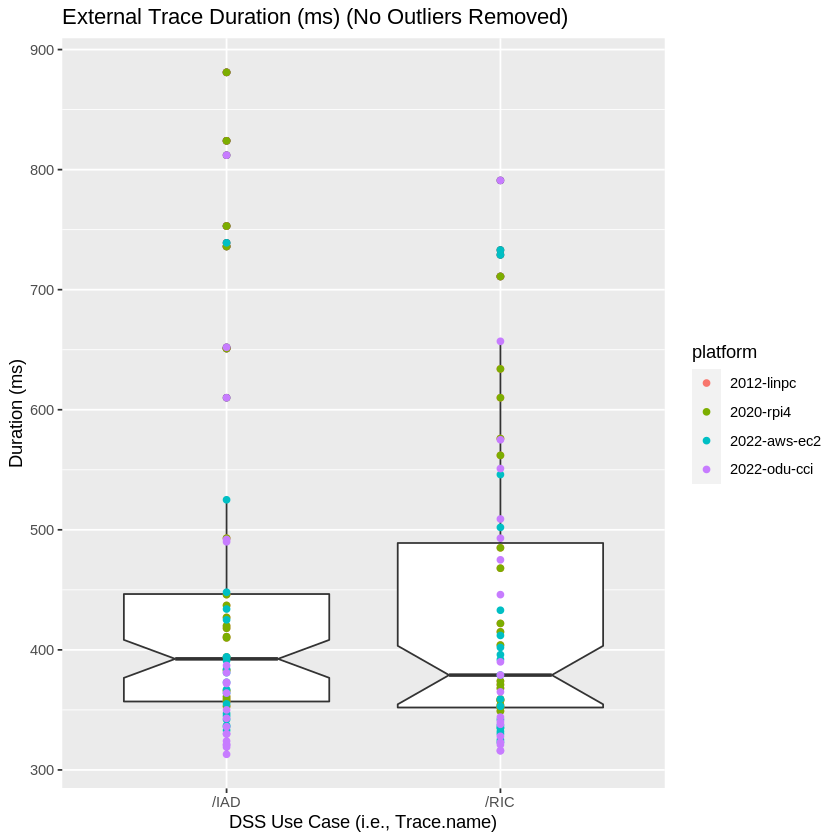
\includegraphics{dss-span-analysis-rev5_files/figure-pdf/cell-61-output-1.png}

}

\end{figure}

\begin{Shaded}
\begin{Highlighting}[]
\NormalTok{eSpan }\SpecialCharTok{\%\textgreater{}\%}
    \FunctionTok{ggplot}\NormalTok{(}\FunctionTok{aes}\NormalTok{(Duration)) }\SpecialCharTok{+} \FunctionTok{geom\_histogram}\NormalTok{(}\AttributeTok{binwidth =} \DecValTok{50}\NormalTok{) }\SpecialCharTok{+}
    \FunctionTok{ggtitle}\NormalTok{(}\StringTok{"External Duration (ms) Histogram (No Outliers Removed), Binwidth = 50ms"}\NormalTok{) }\SpecialCharTok{+}
    \FunctionTok{xlab}\NormalTok{(}\StringTok{"External Duration (ms)"}\NormalTok{)}
\end{Highlighting}
\end{Shaded}

\begin{figure}[H]

{\centering 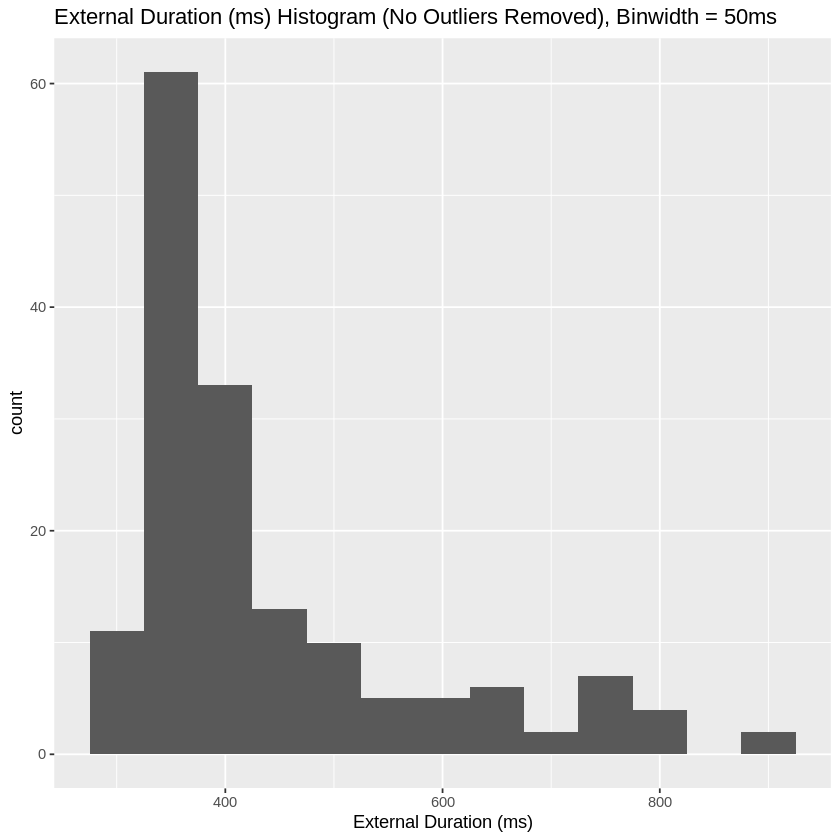
\includegraphics{dss-span-analysis-rev5_files/figure-pdf/cell-62-output-1.png}

}

\end{figure}

Note that the histogram plot of the external data indicates that the
data is not normally distributed and will need a transformation to
enable application of statistics.

\hypertarget{transformation-and-normality-testing-of-the-data}{%
\section{Transformation and Normality Testing of the
Data}\label{transformation-and-normality-testing-of-the-data}}

The histograms of the internal and external span data imply that a log
transform is needed; however, we need to look at cube and sqrt
transforms. A Box-Cox transformation may also need to be explored. Once
that data has been transformed, we shall use a Shapiro-Wilk test to
assess whether or not the data is normally distributed.

\hypertarget{box-cox-transformation}{%
\subsection{Box-Cox Transformation}\label{box-cox-transformation}}

Box and Cox (1964) developed a family of transformations designed to
reduce nonnormality of the errors in a linear model. Applying this
transform often reduces non-linearity as well, and heteroscedascity.

The idea is to transform the response variable \(Y\) to a replacement
response variable \(Y_i^{(\lambda)}\), leaving the right-hand side of
the regression model unchanged, so that the regression residuals become
normally-distributed. Note that the regression coefficients will also
change, because the response variable has changed; therefore, the
regression coefficients must be interpreted with respect to the
transformed variable. Also, any predictions made with the model have to
be back-transformed, to be interpreted in the original units.

The standard (simple) Box-Cox transform is:

\[
    Y_i^{(\lambda)}=
\begin{cases}
{\frac {Y_i^\lambda - 1} \lambda},  & {(\lambda \neq 0)} \\
log(Y_i), & {(\lambda = 0)}
\end{cases}
\]

\emph{Box, G. E. P., \& Cox, D. R. (1964). An Analysis of
Transformations. Journal of the Royal Statistical Society, Series B
(Metholodogical), 26(2), 211-252.}

http://www.css.cornell.edu/faculty/dgr2/\_static/files/R\_html/Transformations.html

\hypertarget{shapiro-wilk-test}{%
\subsection{Shapiro-Wilk Test}\label{shapiro-wilk-test}}

The null-hypothesis of this test is that the population is normally
distributed. Thus, if the p value is less than the chosen alpha level,
then the null hypothesis is rejected and there is evidence that the data
tested are not normally distributed. On the other hand, if the p value
is greater than the chosen alpha level, then the null hypothesis (that
the data came from a normally distributed population) can not be
rejected (e.g., for an alpha level of .05, a data set with a p value of
less than .05 rejects the null hypothesis that the data are from a
normally distributed population).

https://en.wikipedia.org/wiki/Shapiro--Wilk\_test

\hypertarget{data-transformations-and-hypothesis-testing-internal-data}{%
\subsection{Data Transformations and Hypothesis Testing (Internal
Data)}\label{data-transformations-and-hypothesis-testing-internal-data}}

\begin{Shaded}
\begin{Highlighting}[]
\FunctionTok{qqnorm}\NormalTok{(iSpan}\SpecialCharTok{$}\NormalTok{Duration, }\AttributeTok{main=}\StringTok{"Internal Span Duration Q{-}Q Norm Plot"}\NormalTok{)}
\FunctionTok{qqline}\NormalTok{(iSpan}\SpecialCharTok{$}\NormalTok{Duration)}
\end{Highlighting}
\end{Shaded}

\begin{figure}[H]

{\centering 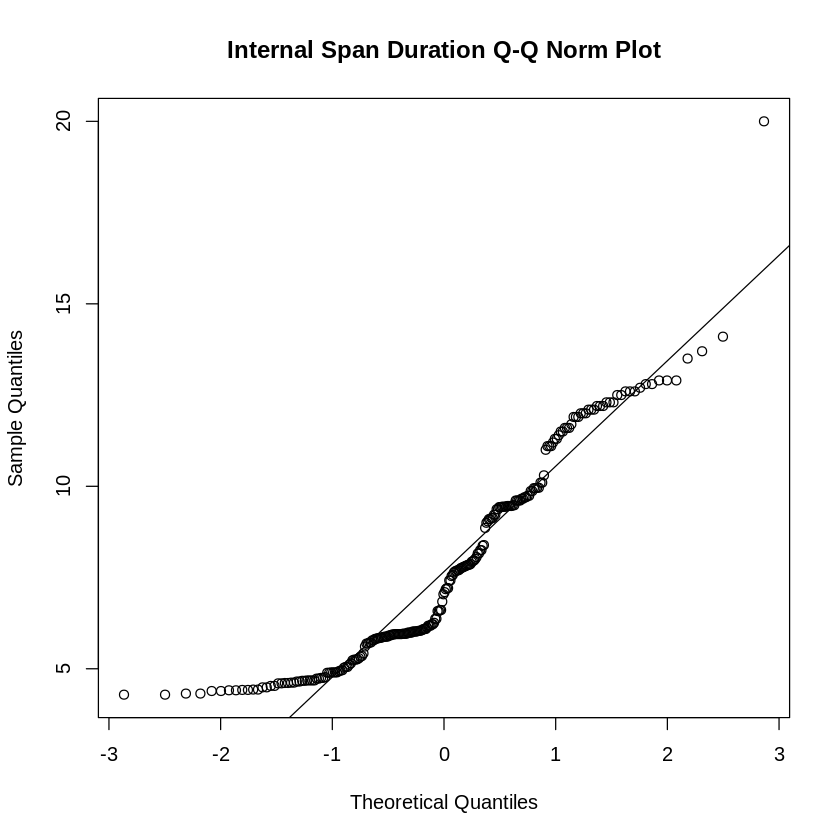
\includegraphics{dss-span-analysis-rev5_files/figure-pdf/cell-63-output-1.png}

}

\end{figure}

\hypertarget{sqrt-log-cube-transformations}{%
\subsubsection{Sqrt-Log-Cube
Transformations}\label{sqrt-log-cube-transformations}}

\begin{Shaded}
\begin{Highlighting}[]
\NormalTok{sqrt\_iSpan }\OtherTok{\textless{}{-}}\NormalTok{ iSpan}
\NormalTok{sqrt\_iSpan}\SpecialCharTok{$}\NormalTok{Duration}\OtherTok{=}\FunctionTok{sqrt}\NormalTok{(sqrt\_iSpan}\SpecialCharTok{$}\NormalTok{Duration)}

\NormalTok{log\_iSpan }\OtherTok{\textless{}{-}}\NormalTok{ iSpan}
\NormalTok{log\_iSpan}\SpecialCharTok{$}\NormalTok{Duration}\OtherTok{=}\FunctionTok{log}\NormalTok{(log\_iSpan}\SpecialCharTok{$}\NormalTok{Duration }\SpecialCharTok{+} \DecValTok{1}\NormalTok{) }\CommentTok{\# Natural Log}
\NormalTok{log10\_iSpan }\OtherTok{\textless{}{-}}\NormalTok{ iSpan}
\NormalTok{log10\_iSpan}\SpecialCharTok{$}\NormalTok{Duration}\OtherTok{=}\FunctionTok{log10}\NormalTok{(log10\_iSpan}\SpecialCharTok{$}\NormalTok{Duration }\SpecialCharTok{+} \DecValTok{1}\NormalTok{) }\CommentTok{\# Log Base 10}
\NormalTok{log2\_iSpan }\OtherTok{\textless{}{-}}\NormalTok{ iSpan}
\NormalTok{log2\_iSpan}\SpecialCharTok{$}\NormalTok{Duration}\OtherTok{=}\FunctionTok{log2}\NormalTok{(log2\_iSpan}\SpecialCharTok{$}\NormalTok{Duration }\SpecialCharTok{+} \DecValTok{1}\NormalTok{) }\CommentTok{\# Log Base 2}

\NormalTok{cube\_iSpan }\OtherTok{\textless{}{-}}\NormalTok{ iSpan}
\NormalTok{cube\_iSpan}\SpecialCharTok{$}\NormalTok{Duration}\OtherTok{=}\NormalTok{cube\_iSpan}\SpecialCharTok{$}\NormalTok{Duration}\SpecialCharTok{\^{}}\NormalTok{(}\DecValTok{1}\SpecialCharTok{/}\DecValTok{3}\NormalTok{)}

\FunctionTok{par}\NormalTok{(}\AttributeTok{mfrow=}\FunctionTok{c}\NormalTok{(}\DecValTok{2}\NormalTok{,}\DecValTok{2}\NormalTok{))}
\FunctionTok{hist}\NormalTok{(iSpan}\SpecialCharTok{$}\NormalTok{Duration, }\AttributeTok{counts =} \DecValTok{10}\NormalTok{)}
\FunctionTok{hist}\NormalTok{(log\_iSpan}\SpecialCharTok{$}\NormalTok{Duration)}
\FunctionTok{hist}\NormalTok{(log10\_iSpan}\SpecialCharTok{$}\NormalTok{Duration)}
\FunctionTok{hist}\NormalTok{(log2\_iSpan}\SpecialCharTok{$}\NormalTok{Duration)}
\end{Highlighting}
\end{Shaded}

\begin{figure}[H]

{\centering 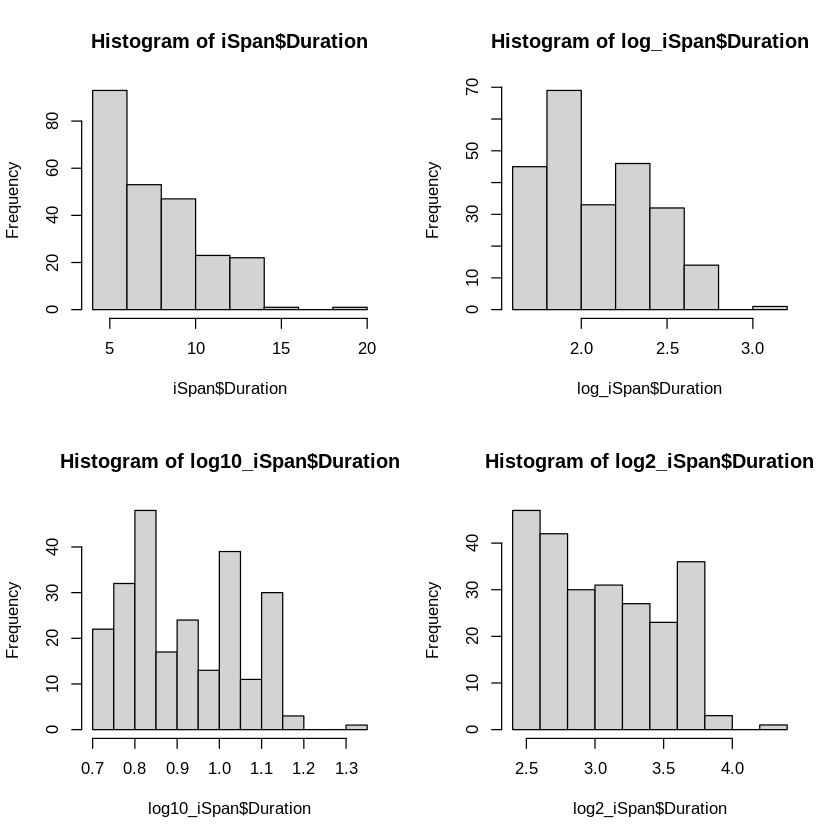
\includegraphics{dss-span-analysis-rev5_files/figure-pdf/cell-64-output-1.png}

}

\end{figure}

\hypertarget{box-cox-transformation-1}{%
\subsubsection{Box-Cox Transformation}\label{box-cox-transformation-1}}

\begin{Shaded}
\begin{Highlighting}[]
\FunctionTok{library}\NormalTok{(}\StringTok{"MASS"}\NormalTok{)}
\end{Highlighting}
\end{Shaded}

\begin{Shaded}
\begin{Highlighting}[]
\NormalTok{bc\_iSpan }\OtherTok{=}\NormalTok{ iSpan}
\NormalTok{x }\OtherTok{\textless{}{-}}\NormalTok{ bc\_iSpan}\SpecialCharTok{$}\NormalTok{Duration}
\NormalTok{bc }\OtherTok{=} \FunctionTok{boxcox}\NormalTok{(}\FunctionTok{lm}\NormalTok{(x }\SpecialCharTok{\textasciitilde{}} \DecValTok{1}\NormalTok{), }\FunctionTok{seq}\NormalTok{(}\SpecialCharTok{{-}}\DecValTok{1}\NormalTok{,}\DecValTok{1}\NormalTok{,.}\DecValTok{1}\NormalTok{))}
\CommentTok{\# bc = boxcox(lm(x \textasciitilde{} bcData$useCaseNum))}
\NormalTok{lambda }\OtherTok{\textless{}{-}}\NormalTok{ bc}\SpecialCharTok{$}\NormalTok{x[}\FunctionTok{which.max}\NormalTok{(bc}\SpecialCharTok{$}\NormalTok{y)]}
\NormalTok{new\_x\_exact }\OtherTok{\textless{}{-}}\NormalTok{ (x }\SpecialCharTok{\^{}}\NormalTok{ lambda }\SpecialCharTok{{-}} \DecValTok{1}\NormalTok{) }\SpecialCharTok{/}\NormalTok{ lambda}
\end{Highlighting}
\end{Shaded}

\begin{figure}[H]

{\centering 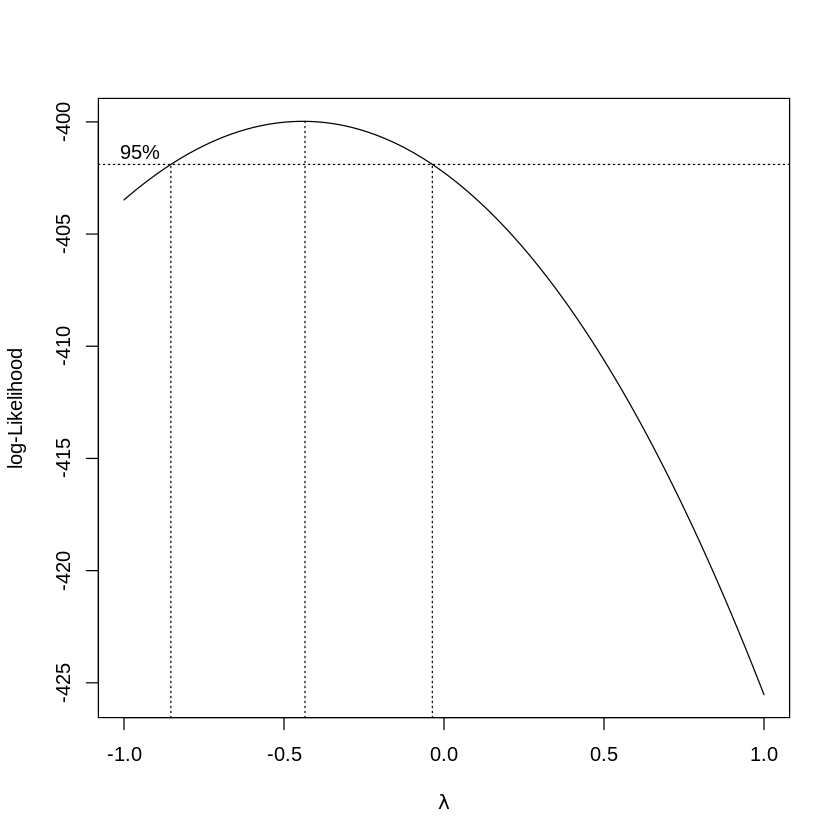
\includegraphics{dss-span-analysis-rev5_files/figure-pdf/cell-66-output-1.png}

}

\end{figure}

\begin{Shaded}
\begin{Highlighting}[]
\NormalTok{bc\_iSpan}\SpecialCharTok{$}\NormalTok{Duration }\OtherTok{=}\NormalTok{ new\_x\_exact}
\FunctionTok{par}\NormalTok{(}\AttributeTok{mfrow=}\FunctionTok{c}\NormalTok{(}\DecValTok{1}\NormalTok{,}\DecValTok{3}\NormalTok{))}
\FunctionTok{hist}\NormalTok{(iSpan}\SpecialCharTok{$}\NormalTok{Duration)}
\FunctionTok{hist}\NormalTok{(bc\_iSpan}\SpecialCharTok{$}\NormalTok{Duration)}
\end{Highlighting}
\end{Shaded}

\begin{figure}[H]

{\centering 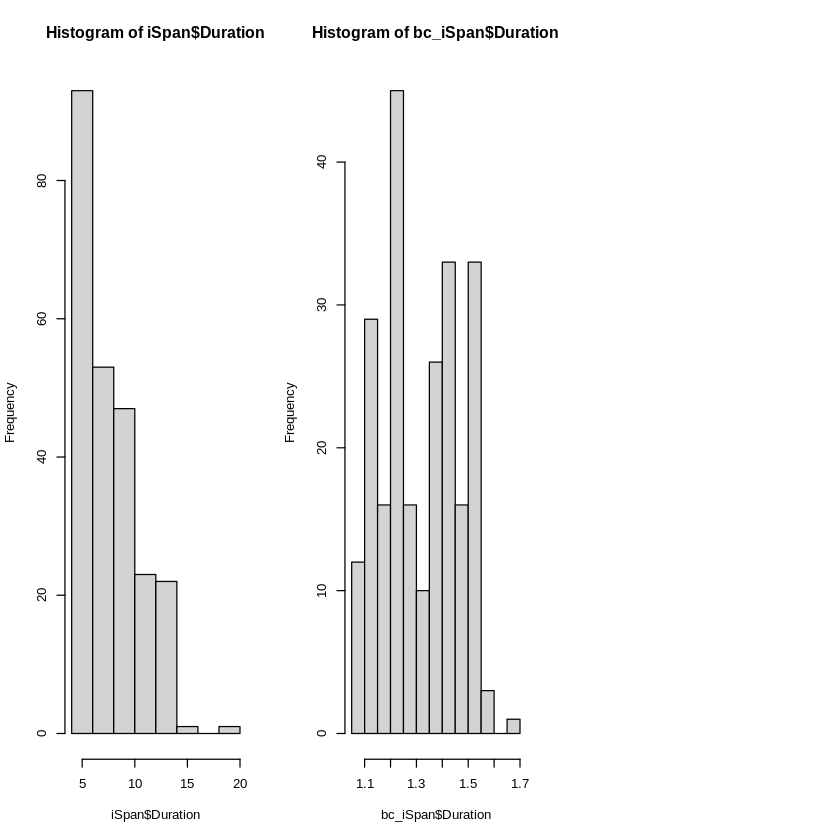
\includegraphics{dss-span-analysis-rev5_files/figure-pdf/cell-67-output-1.png}

}

\end{figure}

\begin{Shaded}
\begin{Highlighting}[]
\NormalTok{? shapiro.test}
\end{Highlighting}
\end{Shaded}

\inputencoding{utf8}
\HeaderA{shapiro.test}{Shapiro-Wilk Normality Test}{shapiro.test}
\keyword{htest}{shapiro.test}
%
\begin{Description}\relax
Performs the Shapiro-Wilk test of normality.
\end{Description}
%
\begin{Usage}
\begin{verbatim}
shapiro.test(x)
\end{verbatim}
\end{Usage}
%
\begin{Arguments}
\begin{ldescription}
\item[\code{x}] a numeric vector of data values. Missing values are allowed,
but the number of non-missing values must be between 3 and 5000.
\end{ldescription}
\end{Arguments}
%
\begin{Value}
A list with class \code{"htest"} containing the following components:
\begin{ldescription}
\item[\code{statistic}] the value of the Shapiro-Wilk statistic.
\item[\code{p.value}] an approximate p-value for the test.  This is
said in Royston (1995) to be adequate for \code{p.value < 0.1}.
\item[\code{method}] the character string \code{"Shapiro-Wilk normality test"}.
\item[\code{data.name}] a character string giving the name(s) of the data.
\end{ldescription}
\end{Value}
%
\begin{Source}\relax
The algorithm used is a C translation of the Fortran code described in
Royston (1995). 
The calculation of the p value is exact for \eqn{n = 3}{}, otherwise
approximations are used, separately for \eqn{4 \le n \le 11}{} and
\eqn{n \ge 12}{}.
\end{Source}
%
\begin{References}\relax
Patrick Royston (1982).
An extension of Shapiro and Wilk's \eqn{W}{} test for normality to large
samples.
\emph{Applied Statistics}, \bold{31}, 115--124.
doi:\nobreakspace{}\Rhref{https://doi.org/10.2307/2347973}{10.2307\slash{}2347973}.

Patrick Royston (1982).
Algorithm AS 181: The \eqn{W}{} test for Normality.
\emph{Applied Statistics}, \bold{31}, 176--180.
doi:\nobreakspace{}\Rhref{https://doi.org/10.2307/2347986}{10.2307\slash{}2347986}.

Patrick Royston (1995).
Remark AS R94: A remark on Algorithm AS 181: The \eqn{W}{} test for
normality.
\emph{Applied Statistics}, \bold{44}, 547--551.
doi:\nobreakspace{}\Rhref{https://doi.org/10.2307/2986146}{10.2307\slash{}2986146}.
\end{References}
%
\begin{SeeAlso}\relax
\code{\LinkA{qqnorm}{qqnorm}} for producing a normal quantile-quantile plot.
\end{SeeAlso}
%
\begin{Examples}
\begin{ExampleCode}
shapiro.test(rnorm(100, mean = 5, sd = 3))
shapiro.test(runif(100, min = 2, max = 4))
\end{ExampleCode}
\end{Examples}

\hypertarget{shapiro-wilk-normality-test}{%
\subsubsection{Shapiro-Wilk Normality
Test}\label{shapiro-wilk-normality-test}}

\begin{Shaded}
\begin{Highlighting}[]
\FunctionTok{shapiro.test}\NormalTok{(iSpan}\SpecialCharTok{$}\NormalTok{Duration)}

\FunctionTok{shapiro.test}\NormalTok{(log\_iSpan}\SpecialCharTok{$}\NormalTok{Duration)}
\FunctionTok{shapiro.test}\NormalTok{(log10\_iSpan}\SpecialCharTok{$}\NormalTok{Duration)}
\FunctionTok{shapiro.test}\NormalTok{(log2\_iSpan}\SpecialCharTok{$}\NormalTok{Duration)}

\FunctionTok{shapiro.test}\NormalTok{(sqrt\_iSpan}\SpecialCharTok{$}\NormalTok{Duration)}
\FunctionTok{shapiro.test}\NormalTok{(cube\_iSpan}\SpecialCharTok{$}\NormalTok{Duration)}

\FunctionTok{shapiro.test}\NormalTok{(bc\_iSpan}\SpecialCharTok{$}\NormalTok{Duration)}
\end{Highlighting}
\end{Shaded}

\begin{verbatim}

    Shapiro-Wilk normality test

data:  iSpan$Duration
W = 0.9075, p-value = 5.081e-11
\end{verbatim}

\begin{verbatim}

    Shapiro-Wilk normality test

data:  log_iSpan$Duration
W = 0.94087, p-value = 2.892e-08
\end{verbatim}

\begin{verbatim}

    Shapiro-Wilk normality test

data:  log10_iSpan$Duration
W = 0.94087, p-value = 2.892e-08
\end{verbatim}

\begin{verbatim}

    Shapiro-Wilk normality test

data:  log2_iSpan$Duration
W = 0.94087, p-value = 2.892e-08
\end{verbatim}

\begin{verbatim}

    Shapiro-Wilk normality test

data:  sqrt_iSpan$Duration
W = 0.93106, p-value = 3.692e-09
\end{verbatim}

\begin{verbatim}

    Shapiro-Wilk normality test

data:  cube_iSpan$Duration
W = 0.93634, p-value = 1.092e-08
\end{verbatim}

\begin{verbatim}

    Shapiro-Wilk normality test

data:  bc_iSpan$Duration
W = 0.9466, p-value = 1.06e-07
\end{verbatim}

With all p-values of \_\_\_\_\_ \textless{} 0.05 we fail reject the null
hypothesis and assume we do not have a normal distribution. We will try
a Box-Cox Transformation.

\emph{``if the p value is greater than the chosen alpha level, then the
null hypothesis (that the data came from a normally distributed
population) can not be rejected''}

\hypertarget{hypothesis-testing-need-to-correct-issue}{%
\subsubsection{Hypothesis Testing (Need to Correct
Issue)}\label{hypothesis-testing-need-to-correct-issue}}

We will use a Student's t-Test to test the hypothesis on \textbf{normal}
internal span data. Our mean is 500 ms (e.g.~\(\mu = 0.5\) seconds) and
our null hypthesis is less than 500 ms.

\begin{Shaded}
\begin{Highlighting}[]
\NormalTok{mu }\OtherTok{=} \FloatTok{0.5}
\NormalTok{x }\OtherTok{=}\NormalTok{ cube\_iSpan}\SpecialCharTok{$}\NormalTok{Duration}
\NormalTok{cube\_mu }\OtherTok{=}\NormalTok{ mu}\SpecialCharTok{\^{}}\NormalTok{(}\DecValTok{1}\SpecialCharTok{/}\DecValTok{3}\NormalTok{)}
\FunctionTok{t.test}\NormalTok{(}\AttributeTok{x=}\NormalTok{x, }\AttributeTok{mu=}\NormalTok{cube\_mu, }\AttributeTok{alternative =} \StringTok{\textquotesingle{}greater\textquotesingle{}}\NormalTok{)}
\end{Highlighting}
\end{Shaded}

\begin{verbatim}

    One Sample t-test

data:  x
t = 78.692, df = 239, p-value < 2.2e-16
alternative hypothesis: true mean is greater than 0.7937005
95 percent confidence interval:
 1.927618      Inf
sample estimates:
mean of x 
 1.951922 
\end{verbatim}

With a p-value of \_\_\_ \textgreater{} 0.05 we reject the null
hypothesis, i.e.~we assume that latency will be greater than 500 ms.

\emph{``If the p value is greater than the chosen alpha level, then the
null hypothesis (that latency is \textless{} 500 ms) can not be
rejected''}

\hypertarget{data-transformations-and-hypothesis-testing-external-data}{%
\subsection{Data Transformations and Hypothesis Testing (External
Data)}\label{data-transformations-and-hypothesis-testing-external-data}}

\begin{Shaded}
\begin{Highlighting}[]
\FunctionTok{qqnorm}\NormalTok{(eSpan}\SpecialCharTok{$}\NormalTok{Duration, }\AttributeTok{main=}\StringTok{"External Span Duration Q{-}Q Norm Plot"}\NormalTok{)}
\FunctionTok{qqline}\NormalTok{(eSpan}\SpecialCharTok{$}\NormalTok{Duration)}
\end{Highlighting}
\end{Shaded}

\begin{figure}[H]

{\centering 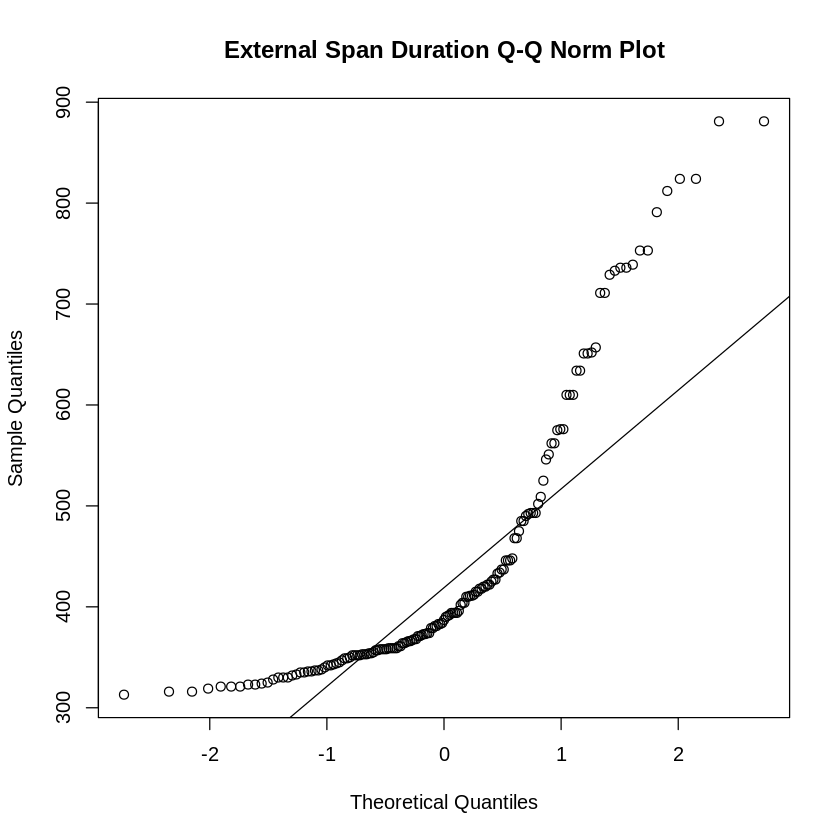
\includegraphics{dss-span-analysis-rev5_files/figure-pdf/cell-71-output-1.png}

}

\end{figure}

\hypertarget{sqrt-log-cube-transformations-1}{%
\subsubsection{Sqrt-Log-Cube
Transformations}\label{sqrt-log-cube-transformations-1}}

\begin{Shaded}
\begin{Highlighting}[]
\NormalTok{sqrt\_eSpan }\OtherTok{\textless{}{-}}\NormalTok{ eSpan}
\NormalTok{sqrt\_eSpan}\SpecialCharTok{$}\NormalTok{Duration}\OtherTok{=}\FunctionTok{sqrt}\NormalTok{(sqrt\_eSpan}\SpecialCharTok{$}\NormalTok{Duration)}

\NormalTok{log\_eSpan }\OtherTok{\textless{}{-}}\NormalTok{ eSpan}
\NormalTok{log\_eSpan}\SpecialCharTok{$}\NormalTok{Duration}\OtherTok{=}\FunctionTok{log}\NormalTok{(log\_eSpan}\SpecialCharTok{$}\NormalTok{Duration }\SpecialCharTok{+} \DecValTok{1}\NormalTok{) }\CommentTok{\# Natural Log}
\NormalTok{log10\_eSpan }\OtherTok{\textless{}{-}}\NormalTok{ eSpan}
\NormalTok{log10\_eSpan}\SpecialCharTok{$}\NormalTok{Duration}\OtherTok{=}\FunctionTok{log10}\NormalTok{(log10\_eSpan}\SpecialCharTok{$}\NormalTok{Duration }\SpecialCharTok{+} \DecValTok{1}\NormalTok{) }\CommentTok{\# Log Base 10}
\NormalTok{log2\_eSpan }\OtherTok{\textless{}{-}}\NormalTok{ iSpan}
\NormalTok{log2\_eSpan}\SpecialCharTok{$}\NormalTok{Duration}\OtherTok{=}\FunctionTok{log2}\NormalTok{(log2\_eSpan}\SpecialCharTok{$}\NormalTok{Duration }\SpecialCharTok{+} \DecValTok{1}\NormalTok{) }\CommentTok{\# Log Base 2}

\NormalTok{cube\_eSpan }\OtherTok{\textless{}{-}}\NormalTok{ eSpan}
\NormalTok{cube\_eSpan}\SpecialCharTok{$}\NormalTok{Duration}\OtherTok{=}\NormalTok{cube\_eSpan}\SpecialCharTok{$}\NormalTok{Duration}\SpecialCharTok{\^{}}\NormalTok{(}\DecValTok{1}\SpecialCharTok{/}\DecValTok{3}\NormalTok{)}

\FunctionTok{par}\NormalTok{(}\AttributeTok{mfrow=}\FunctionTok{c}\NormalTok{(}\DecValTok{2}\NormalTok{,}\DecValTok{2}\NormalTok{))}
\FunctionTok{hist}\NormalTok{(eSpan}\SpecialCharTok{$}\NormalTok{Duration, }\AttributeTok{counts =} \DecValTok{50}\NormalTok{)}
\FunctionTok{hist}\NormalTok{(log\_eSpan}\SpecialCharTok{$}\NormalTok{Duration)}
\FunctionTok{hist}\NormalTok{(log10\_eSpan}\SpecialCharTok{$}\NormalTok{Duration)}
\FunctionTok{hist}\NormalTok{(log2\_eSpan}\SpecialCharTok{$}\NormalTok{Duration)}
\end{Highlighting}
\end{Shaded}

\begin{figure}[H]

{\centering 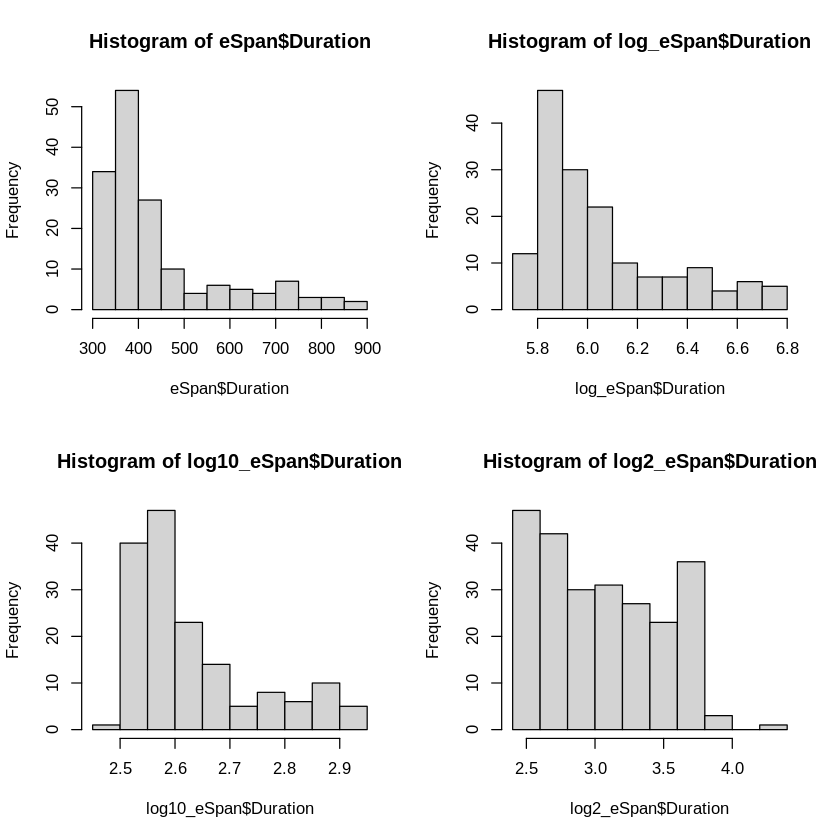
\includegraphics{dss-span-analysis-rev5_files/figure-pdf/cell-72-output-1.png}

}

\end{figure}

\hypertarget{box-cox-transformation-2}{%
\subsubsection{Box-Cox Transformation}\label{box-cox-transformation-2}}

\begin{Shaded}
\begin{Highlighting}[]
\NormalTok{bc\_eSpan }\OtherTok{=}\NormalTok{ eSpan}
\NormalTok{x }\OtherTok{\textless{}{-}}\NormalTok{ bc\_eSpan}\SpecialCharTok{$}\NormalTok{Duration}
\NormalTok{bc }\OtherTok{=} \FunctionTok{boxcox}\NormalTok{(}\FunctionTok{lm}\NormalTok{(x }\SpecialCharTok{\textasciitilde{}} \DecValTok{1}\NormalTok{), }\FunctionTok{seq}\NormalTok{(}\SpecialCharTok{{-}}\DecValTok{3}\NormalTok{,}\DecValTok{3}\NormalTok{,.}\DecValTok{1}\NormalTok{))}
\CommentTok{\# bc = boxcox(lm(x \textasciitilde{} bcData$useCaseNum))}
\NormalTok{lambda }\OtherTok{\textless{}{-}}\NormalTok{ bc}\SpecialCharTok{$}\NormalTok{x[}\FunctionTok{which.max}\NormalTok{(bc}\SpecialCharTok{$}\NormalTok{y)]}
\NormalTok{new\_x\_exact }\OtherTok{\textless{}{-}}\NormalTok{ (x }\SpecialCharTok{\^{}}\NormalTok{ lambda }\SpecialCharTok{{-}} \DecValTok{1}\NormalTok{) }\SpecialCharTok{/}\NormalTok{ lambda}
\end{Highlighting}
\end{Shaded}

\begin{figure}[H]

{\centering 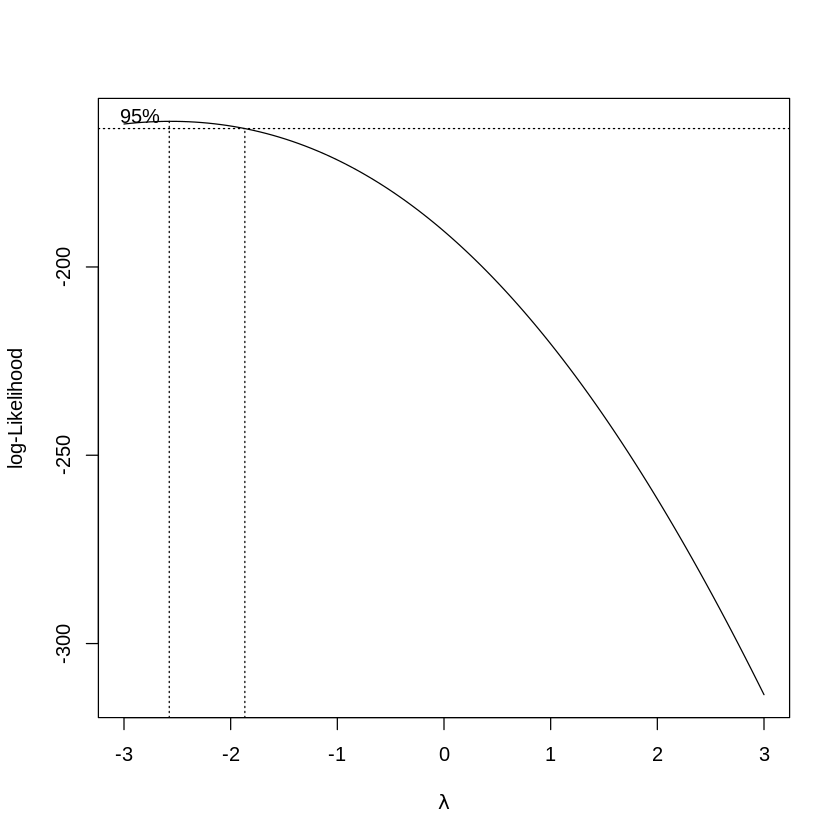
\includegraphics{dss-span-analysis-rev5_files/figure-pdf/cell-73-output-1.png}

}

\end{figure}

\begin{Shaded}
\begin{Highlighting}[]
\NormalTok{bc\_eSpan}\SpecialCharTok{$}\NormalTok{Duration }\OtherTok{=}\NormalTok{ new\_x\_exact}
\FunctionTok{par}\NormalTok{(}\AttributeTok{mfrow=}\FunctionTok{c}\NormalTok{(}\DecValTok{1}\NormalTok{,}\DecValTok{3}\NormalTok{))}
\FunctionTok{hist}\NormalTok{(eSpan}\SpecialCharTok{$}\NormalTok{Duration)}
\FunctionTok{hist}\NormalTok{(bc\_eSpan}\SpecialCharTok{$}\NormalTok{Duration)}
\end{Highlighting}
\end{Shaded}

\begin{figure}[H]

{\centering 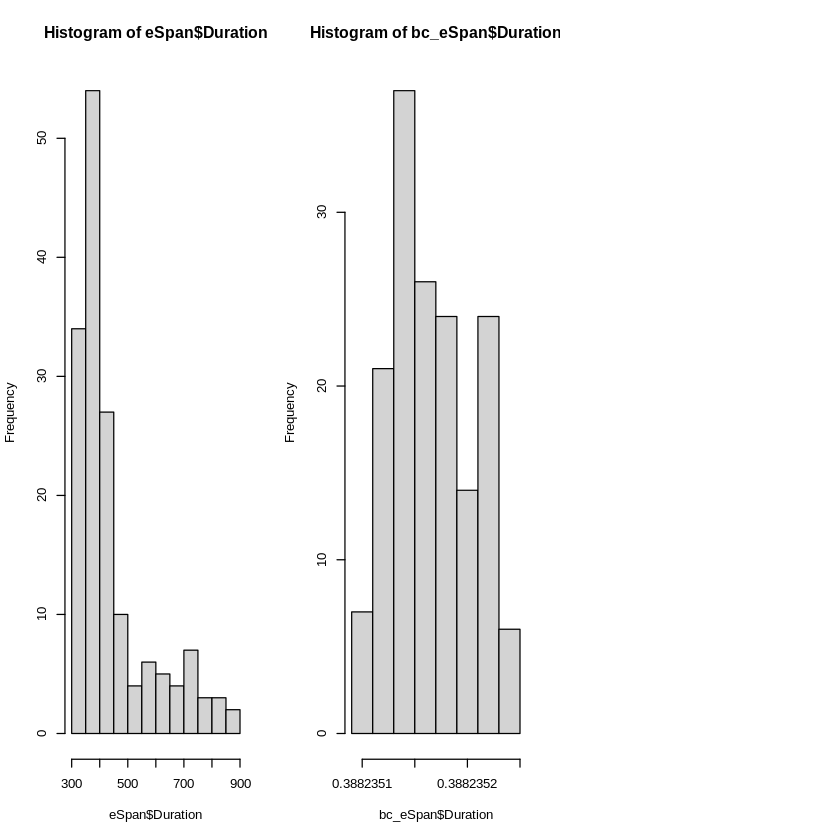
\includegraphics{dss-span-analysis-rev5_files/figure-pdf/cell-74-output-1.png}

}

\end{figure}

\hypertarget{shapiro-wilk-normality-test-1}{%
\subsubsection{Shapiro-Wilk Normality
Test}\label{shapiro-wilk-normality-test-1}}

\begin{Shaded}
\begin{Highlighting}[]
\FunctionTok{shapiro.test}\NormalTok{(eSpan}\SpecialCharTok{$}\NormalTok{Duration)}

\FunctionTok{shapiro.test}\NormalTok{(log\_eSpan}\SpecialCharTok{$}\NormalTok{Duration)}
\FunctionTok{shapiro.test}\NormalTok{(log10\_eSpan}\SpecialCharTok{$}\NormalTok{Duration)}
\FunctionTok{shapiro.test}\NormalTok{(log2\_eSpan}\SpecialCharTok{$}\NormalTok{Duration)}

\FunctionTok{shapiro.test}\NormalTok{(sqrt\_eSpan}\SpecialCharTok{$}\NormalTok{Duration)}
\FunctionTok{shapiro.test}\NormalTok{(cube\_eSpan}\SpecialCharTok{$}\NormalTok{Duration)}

\FunctionTok{shapiro.test}\NormalTok{(bc\_eSpan}\SpecialCharTok{$}\NormalTok{Duration)}
\end{Highlighting}
\end{Shaded}

\begin{verbatim}

    Shapiro-Wilk normality test

data:  eSpan$Duration
W = 0.78293, p-value = 4.439e-14
\end{verbatim}

\begin{verbatim}

    Shapiro-Wilk normality test

data:  log_eSpan$Duration
W = 0.85298, p-value = 2.506e-11
\end{verbatim}

\begin{verbatim}

    Shapiro-Wilk normality test

data:  log10_eSpan$Duration
W = 0.85298, p-value = 2.506e-11
\end{verbatim}

\begin{verbatim}

    Shapiro-Wilk normality test

data:  log2_eSpan$Duration
W = 0.94087, p-value = 2.892e-08
\end{verbatim}

\begin{verbatim}

    Shapiro-Wilk normality test

data:  sqrt_eSpan$Duration
W = 0.81964, p-value = 9.941e-13
\end{verbatim}

\begin{verbatim}

    Shapiro-Wilk normality test

data:  cube_eSpan$Duration
W = 0.83121, p-value = 2.898e-12
\end{verbatim}

\begin{verbatim}

    Shapiro-Wilk normality test

data:  bc_eSpan$Duration
W = 0.95268, p-value = 3.266e-05
\end{verbatim}

With a p-value of \_\_\_\_\_ \textless{} 0.05 we reject the null
hypothesis, i.e.~we assume that we do not have a normal distribution.

\emph{``if the p value is greater than the chosen alpha level, then the
null hypothesis (that the data came from a normally distributed
population) can not be rejected''}

\hypertarget{hypothesis-testing-update-and-correct}{%
\subsubsection{Hypothesis Testing (Update and
Correct)}\label{hypothesis-testing-update-and-correct}}

We will use a Student's t-Test to test the hypothesis on external span
data. Our mean is 500 ms (e.g.~\(\mu = 0.5\) seconds) and our null
hypthesis is less than 500 ms.

\begin{Shaded}
\begin{Highlighting}[]
\NormalTok{mu }\OtherTok{=} \FloatTok{0.5}
\end{Highlighting}
\end{Shaded}

\begin{Shaded}
\begin{Highlighting}[]
\NormalTok{x }\OtherTok{=}\NormalTok{ eSpan}\SpecialCharTok{$}\NormalTok{Duration}
\FunctionTok{t.test}\NormalTok{(}\AttributeTok{x=}\NormalTok{x, }\AttributeTok{mu=}\NormalTok{mu, }\AttributeTok{alternative =} \StringTok{\textquotesingle{}greater\textquotesingle{}}\NormalTok{)}
\end{Highlighting}
\end{Shaded}

\begin{verbatim}

    One Sample t-test

data:  x
t = 41.115, df = 158, p-value < 2.2e-16
alternative hypothesis: true mean is greater than 0.5
95 percent confidence interval:
 424.4261      Inf
sample estimates:
mean of x 
 442.2013 
\end{verbatim}

With a p-value of \_\_\_\_\_ \textgreater{} 0.05 we fail to reject the
null hypothesis, i.e.~we assume that 500 ms can be maintained for
external service requests.

\emph{``If the p value is greater than the chosen alpha level, then the
null hypothesis (that latency is \textless{} 500 ms) can not be
rejected''}

\hypertarget{observations}{%
\section{Observations}\label{observations}}

\hypertarget{general-discussion-of-normality}{%
\subsection{General Discussion of
Normality}\label{general-discussion-of-normality}}

It was required to separate external data from internal to establish
normality of the data samples. The internal data set required
transformation to establish normality, while the external data did not
require a transformation.

\hypertarget{hypothesis-results-update-to-reflect-results}{%
\subsection{Hypothesis Results (Update to Reflect
Results)}\label{hypothesis-results-update-to-reflect-results}}

Hypothesis testing using the Student's t-Test indicates that latency
constraints of 500 ms can be maintained internally and external.
However, serveral external samples were greater than 500 ms. This is
most likely due to the non-deterministic nature of internet (e.g.~http)
requests. Within the internal environment, data is directly routed
between microservices within the Docker environment within a private
network. The data shows that a container based microservice architecture
can meet the requirement; however, care must be taken to manage
processing per container that may increase container response times.

\hypertarget{dss-prototype-environment}{%
\subsection{DSS Prototype Environment}\label{dss-prototype-environment}}

The non deterministic nature of the Docker environment on the MacBook
laptop significantly affected the ability to assess deterministic
behavior. Boxplots of data inclusive of what was sampled from the
MacBook clearly depicted this issue. Linux platforms truly run a
container as intended; however, non-linux platform require the use of a
Linux based Virtual Machine on top of the host OS to implement
containers. While the MacBook met the needs for rapid software
development, the use of a separate integration and test environment was
clearly validated through the collected data.



\end{document}
